\documentclass[10pt,a4paper]{article}
\usepackage[utf8]{inputenc}
\usepackage[russian]{babel}
\usepackage[OT1]{fontenc}
\usepackage{amsmath}
\usepackage{amsfonts}
\usepackage{amssymb}
\usepackage{graphicx}
\usepackage{placeins}
\graphicspath{{lab4/},{lab5/},{lab6/},{lab7/},{lab8/},{lab9/}}


\author{Климов С.А., Назарова К.Е.}
\title{Отчет по лабораторным работам по дисциплине ТСС}
\date{2014}
\begin{document}
\maketitle
\pagebreak
\tableofcontents
\pagebreak
\section{Система верстки \TeX и расширения \LaTeX}
\subsection{Цель работы}
Изучение принципов верстки ТеХ, создание первого отчета
\subsection{Ход работы}
\paragraph{Изучение}
\begin{enumerate}
\item Создание минимального файла .tex в простом текстовом редакторе - преамбула, тело документа
\item Компиляция в командной строке - latex, xdvi, pdflatex
\item Оболочка TexMaker, Быстрый старт, быстрая сборка
\item Создание титульного листа, нескольких разделов, списка, несложной формулы
\end{enumerate}
\paragraph{Выполнение практического задания}
\begin{displaymath}
c^2 = a^2 + b^2
\end{displaymath}
\begin{equation}
c_1+c_2=b_0\frac{2*a}{\log2}
\sum_{i=0}^{\infty}\Theta
\end{equation}
\begin{equation}
b(k) = (-1)^k\frac{2}{N}\sum_{n=0}^{\frac{N}{2}-1}a(n)cos{\frac{\pi k(2n+1)}{N}}
\end{equation}
\begin{equation}
R_2=\frac{(|A|+1)/(\pi f_c C_1)}{b+\sqrt{b^2-4c(|A|+1)C_2/C_1}}
\end{equation}
\subsection{Выводы}
При выполнении данной работы мы ознакомились с ситемой верстки \TeX  и расширением \LaTeX. Были получены начальные навыки верстки документа, а также построения различного вида формул.
\subsection{Материалы}
\begin{enumerate}
\item Не очень краткое введение
\item Конспект-справочник
\item http://www.inp.nsk.su/~baldin/LaTeX/lurs.pdf
\item Математика в \LaTeX
\end{enumerate}
\subsection{Инструменты}
\begin{enumerate}
\item TeX для Windows ProText
\item TeXnicCenter
\item TeXmaker
\end{enumerate}
\section{Визуализация сигналов во временной и частотной области}
\subsection{Цель работы}
Познакомиться со средствами генерации сигналов и визуализации их спектров.
\subsection{Постановка задачи}
В командном окне MATLAB и в среде Simulink промоделировать чистый синусоидальный сигнал, а также синусоидальный сигнал с шумом. Получить их спектры.
\subsection{Справочные материалы}
В.С. Гутников Фильтрация измерительных сигналов пп.1-2, 11-12
\subsection{Ход работы}
В среде MATLAB вначале моделируем чистый синусоидальный сигнал по формуле:
\begin{displaymath}
A(t) = A_0sin(2\pi ft + f_0)
\end{displaymath}
Затем моделируем зашумленный сигнал по формуле:
\begin{displaymath}
A(t) = A_0sin(2\pi ft + f_0) + A_1 rand()
\end{displaymath}
Для выделения частот регулярных составляющих используем преобразование Фурье, которое реализовано встроенной в MATLAB функцией.
\paragraph{Код MATLAB}
\begin{flushleft}
f = 10;\\
x = 0:0.01:8*pi;\\
y = sin(2*pi*f*x+pi/2);\\
plot(x(1:200),y(1:200))\\
grid\\
figure\\
spectrum = fft(y,512);\\
norm\_spectrum = spectrum.*conj(spectrum)/512;\\
f=100*(0:511)/512;\\
plot(f, norm\_spectrum(1:512))\\
axis([0 max(f) 0 10])\\
grid\\
y\_noise = y + 0.6 * rand(size(x));\\
figure\\
plot(x(1:200),y\_noise(1:200));\\
grid\\
spectrum\_noise = fft(y\_noise,512);\\
noise\_spectrum = spectrum\_noise.*conj(spectrum\_noise)/512;\\
figure\\
plot(f, noise\_spectrum(1:512))\\
axis([0 max(f) 0 10])\\
grid\\
\end{flushleft}
\subsection{Результаты работы}
В результате получаем следующие графики временных и частотных характеристик для чистого и зашумленного синусоидального сигналов:

\begin{figure}[h]
\centering
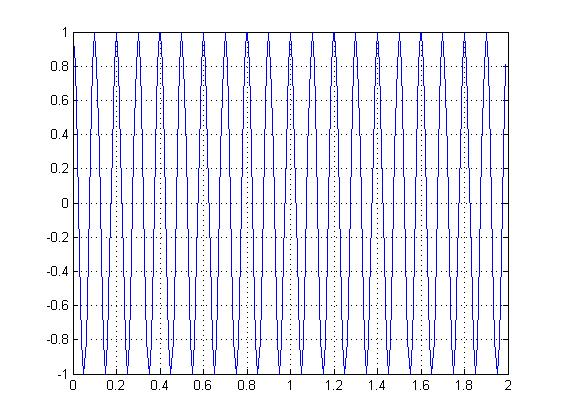
\includegraphics[width=10cm]{1.jpg} 
\caption{Временная характеристика чистого синусоидального сигнала} 
\label{fig.0} 
\end{figure}
\newpage
\begin{figure}[h]
\centering
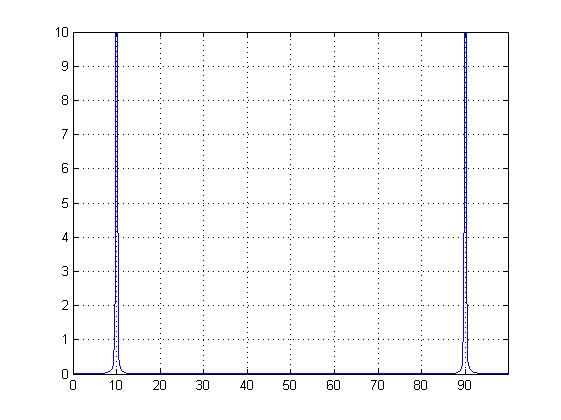
\includegraphics[width=10cm]{2.jpg} 
\caption{Частотная характеристика чистого синусоидального сигнала} 
\label{fig.1} 
\end{figure}
\begin{figure}[h]
\centering
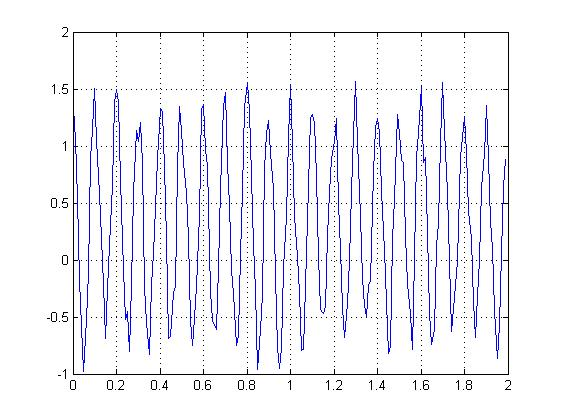
\includegraphics[width=10cm]{3.jpg} 
\caption{Временная характеристика зашумленного синусоидального сигнала} 
\label{fig.2} 
\end{figure}
\newpage
\begin{figure}[h]
\centering
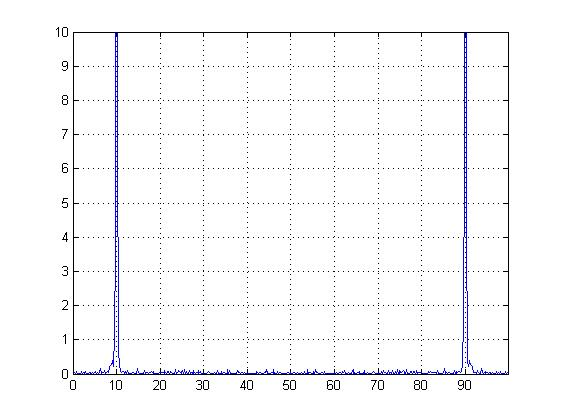
\includegraphics[width=10cm]{4.jpg} 
\caption{Частотная характеристика зашумленного синусоидального сигнала} 
\label{fig.3} 
\end{figure}

\subsection{Выводы}
\newpage
По результатам моделирования синусоидальных сигналов (чистого и с шумом) а также их полученных спектров можно сделать следующие выводы: умноженный на свое комплексное сопряженное спектр является нормированным, синус не бесконечен, спектр испытывает свертку с синком, повторение спектра происходит на частоте, кратной частоте дискретезации.

\newpage
\section{Спектры простых сигналов}
\subsection{Цель работы}
Получить представление о свойствах спектров.
\subsection{Постановка задачи}
В командном окне MATLAB и в среде Simulink промоделировать следующие тестовые сигналы:
\begin{itemize}
\item Полигармонический сигнал 
	\begin{equation}
	y(t) = \sum_{n=0}^{{N}-1}cos{(nt)}
	\end{equation}
\item Прямоугольный импульсный сигнал
	\begin{equation}
	y(t) = \prod(t, T_i)
	\end{equation}
\item Tреугольный импульсный сигнал
	\begin{equation}
	y(t) = \vartriangle(t, T_i)
	\end{equation}
\end{itemize}
и получить их спектры.
\subsection{Справочные материалы}
В.С. Гутников. Фильтрация измерительных сигналов пп.3-6, 13-14
\subsection{Ход работы}
Для моделирования заданных сигналов использовался приведенный код MATLAB:

\begin{verbatim}
t = 0:00.1:4*pi;
N = 100;
y = 0;

% Полигармонический сигнал
y = sin(pi*t)+sin(2*pi*t)+sin(pi*0.3*t);
plot(t,y,'LineWidth',2)
grid

figure
spectrum = fft(y,512);
norm_spectrum = spectrum.*conj(spectrum)/512;
f=100*(0:255)/512;
plot(f, norm_spectrum(1:256),'LineWidth',2)
axis([0 max(f) 0 10])
grid

% Прямоугольный сигнал
figure
y1 = square(t,50);
plot(t(1:100),y1(1:100),'LineWidth',2);
ylim([-2,2]);
grid

figure
spectrum = fft(y1,512);
norm_spectrum = spectrum.*conj(spectrum)/512;
f1=100*(0:255)/512;
plot(f1, norm_spectrum(1:256),'LineWidth',2)
axis([0 max(f1) 0 10])
grid

% Треугольный сигнал
figure
y2 = conv(square(t,20),square(t,20));
plot(t(1:100),y2(1:100),'LineWidth',2);
grid

figure
spectrum = fft(y2,512);
norm\_spectrum = spectrum.*conj(spectrum)/512;
f2=100*(0:255)/512;
plot(f2, norm_spectrum(1:256)/1000,'LineWidth',2)
axis([0 max(f2) 0 50])
grid
\end{verbatim}
\subsection{Результаты работы}
В результате были получены следующие сигналы и их спектры:


\begin{figure}[h]\centering
  \parbox[b]{0.49\textwidth}{\centering
    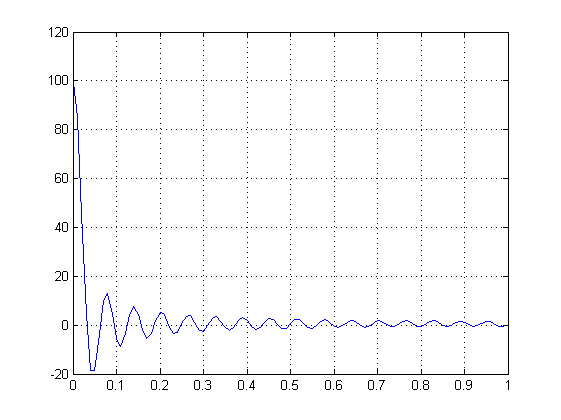
\includegraphics[width=6.5cm]{5_1} 
    \caption{Полигармонический сигнал}\label{fig.l5_1}}
  \hfil\hfil 
  \begin{minipage}[b]{0.49\textwidth}
	\centering
	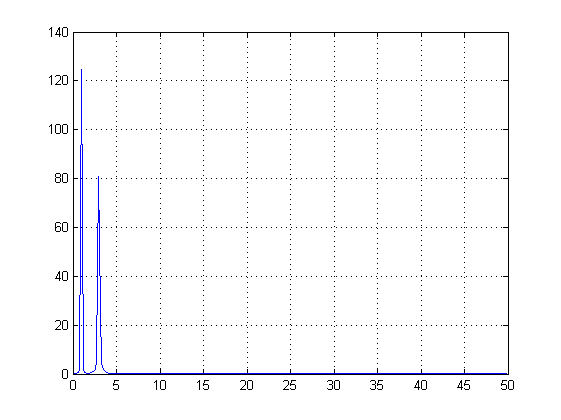
\includegraphics[width=6.5cm]{5_2}
	\caption{Спектр полигармонического сигнала}\label{fig.l5_2} 
  \end{minipage}
\end{figure}

\begin{figure}[h]\centering
  \parbox[b]{0.49\textwidth}{\centering
    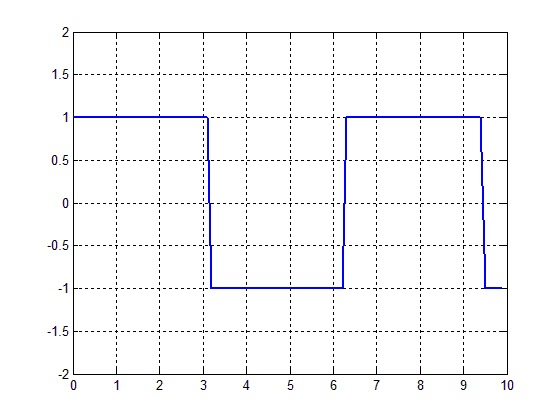
\includegraphics[width=6.5cm]{5_3} 
    \caption{Полигармонический сигнал}\label{fig.l5_3}}
  \hfil\hfil 
  \begin{minipage}[b]{0.49\textwidth}
	\centering
	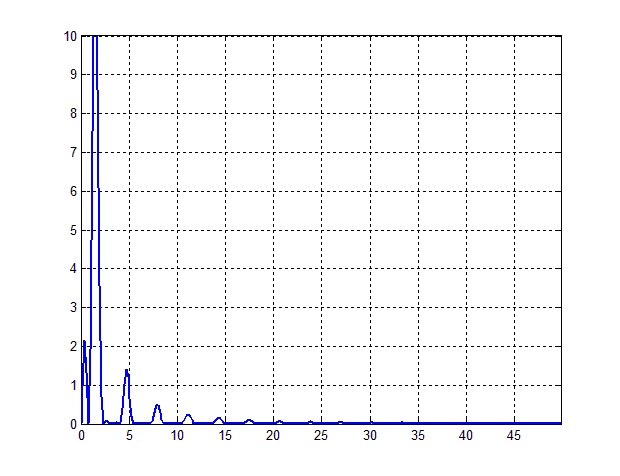
\includegraphics[width=6.5cm]{5_4}
	\caption{Спектр полигармонического сигнала}\label{fig.l5_4} 
  \end{minipage}
\end{figure}

\begin{figure}[h]\centering
  \parbox[b]{0.49\textwidth}{\centering
    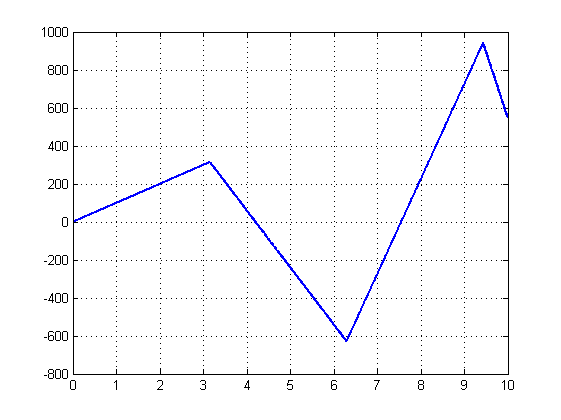
\includegraphics[width=6.5cm]{5_5} 
    \caption{Полигармонический сигнал}\label{fig.l5_5}}
  \hfil\hfil 
  \begin{minipage}[b]{0.49\textwidth}
	\centering
	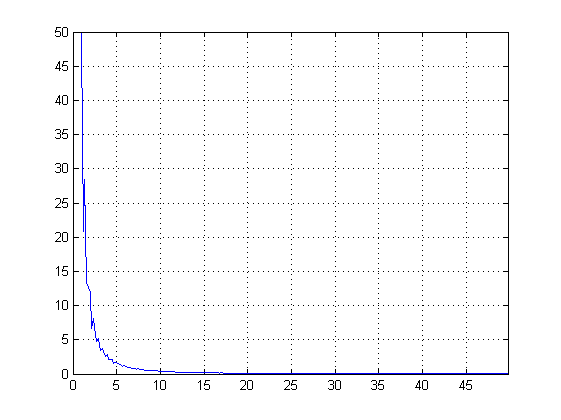
\includegraphics[width=6.5cm]{5_6}
	\caption{Спектр полигармонического сигнала}\label{fig.l5_6} 
  \end{minipage}
\end{figure}

\FloatBarrier

В ходе моделирования сигналов в Simulink были собраны следующие схемы и получены соответствующие графики:


\begin{itemize}
\item Полигармонический сигнал (Рис. 11 - 13)
\begin{figure}[h]
\centering
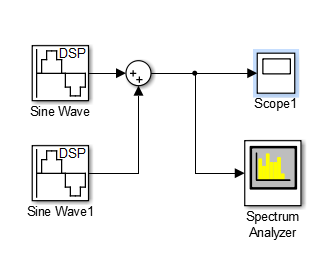
\includegraphics[width=10cm]{1_simulink} 
\caption{Полигармонический сигнал (Simulink)} 
\label{fig.l5_1s} 
\end{figure}
\begin{figure}[h]
\centering
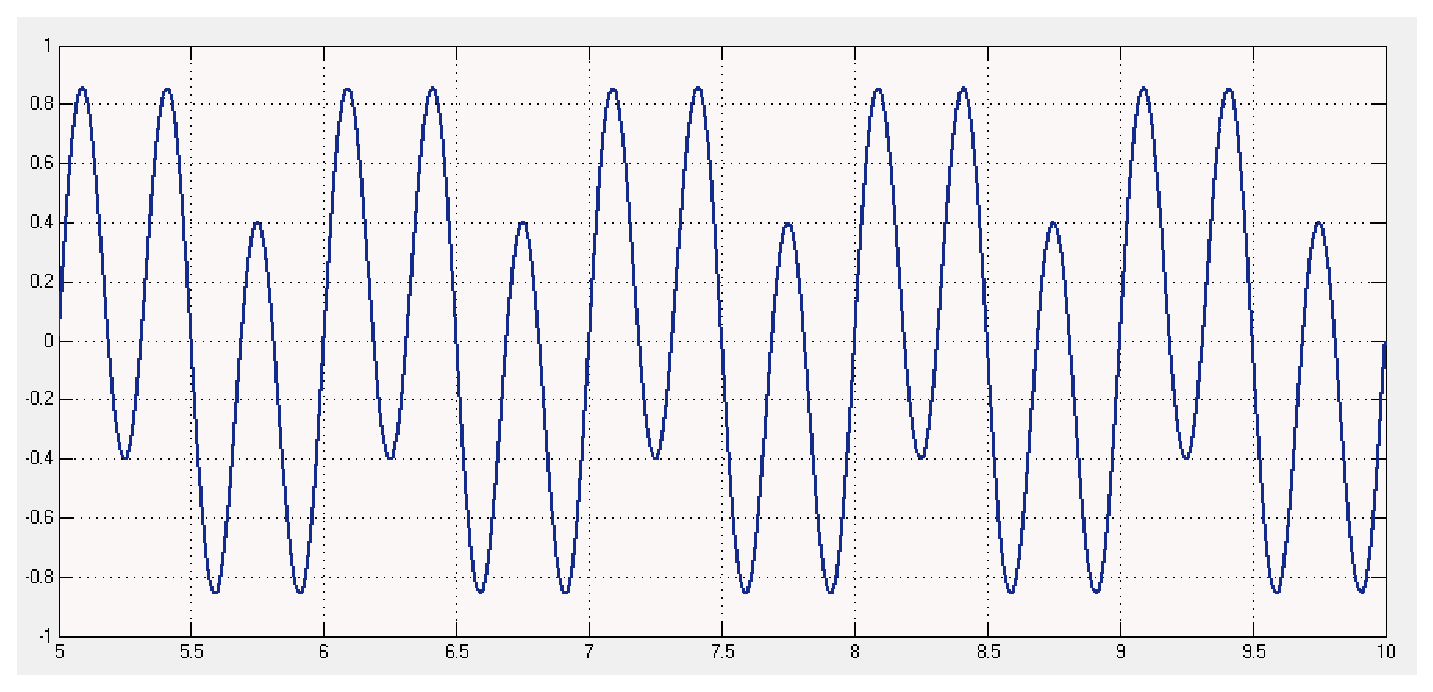
\includegraphics[width=10cm]{lab5_1_simulink} 
\caption{Полигармонический сигнал} 
\label{fig.l5_2s1} 
\end{figure}
\begin{figure}[h]
\centering
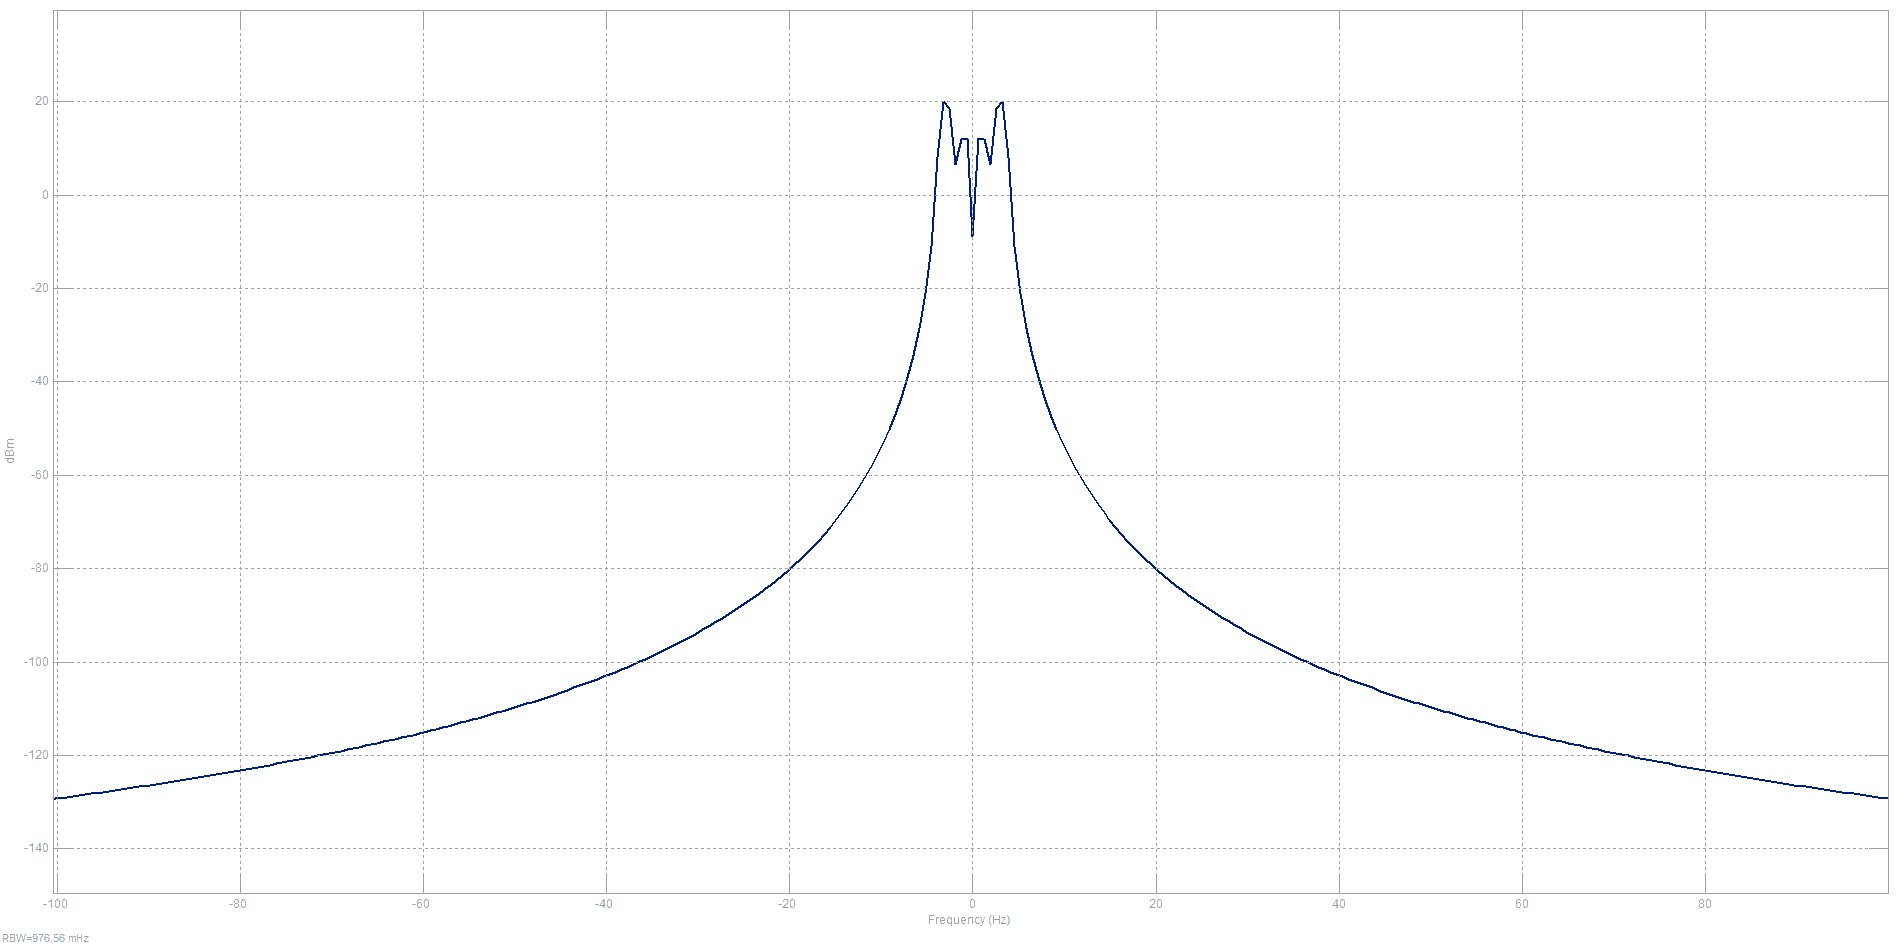
\includegraphics[width=10cm]{lab5_2_simulink}
\caption{Спектр полигармонического сигнала} 
\label{fig.l5_3s} 
\end{figure}

\item Прямоугольный импульсный сигнал (Рис. 14 - 16)
\begin{figure}[h]
\centering
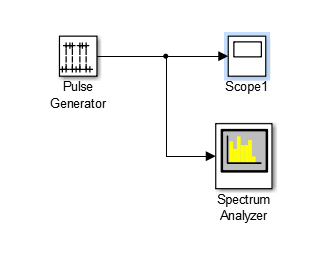
\includegraphics[width=10cm]{3_simulink} 
\caption{Прямоугольный импульсный сигнал (Simulink)} 
\label{fig.l5_4s} 
\end{figure}
\begin{figure}[h]
\centering
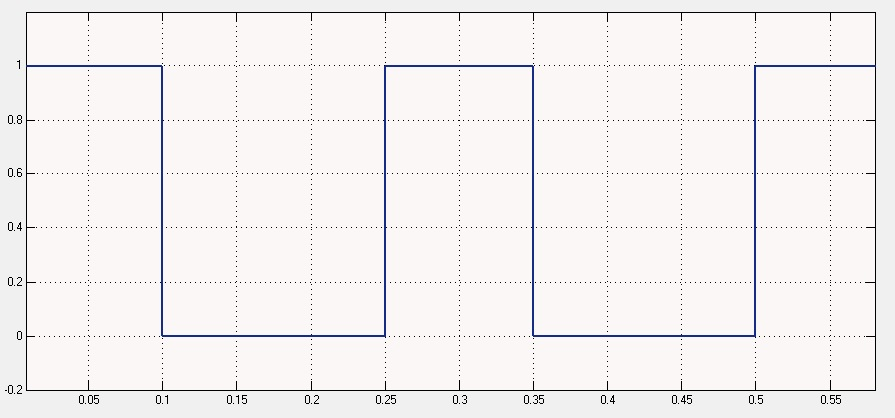
\includegraphics[width=10cm]{lab5_3_simulink} 
\caption{Прямоугольный импульсный сигнал} 
\label{fig.l5_5s} 
\end{figure}
\begin{figure}[h]
\centering
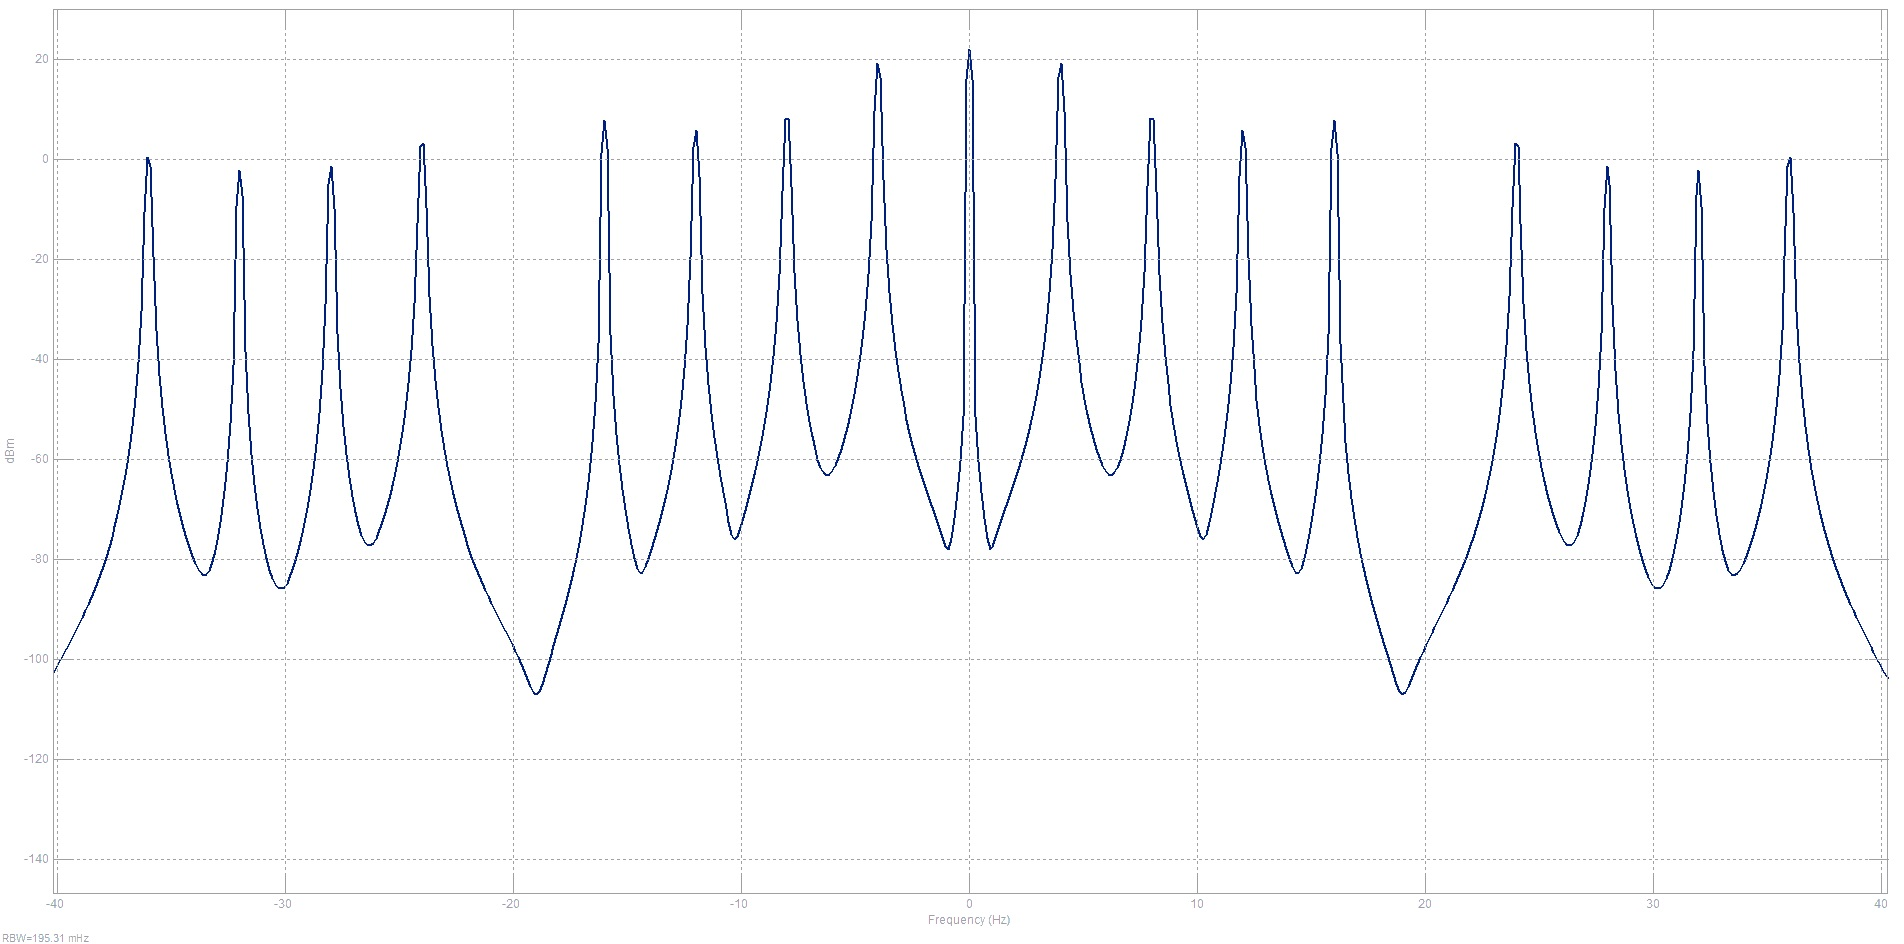
\includegraphics[width=10cm]{lab5_4_simulink}
\caption{Спектр прямоугольного сигнала} 
\label{fig.l5_6s} 
\end{figure}

\item Треугольный импульсный сигнал (Рис. 17 - 19)
\begin{figure}[h]
\centering
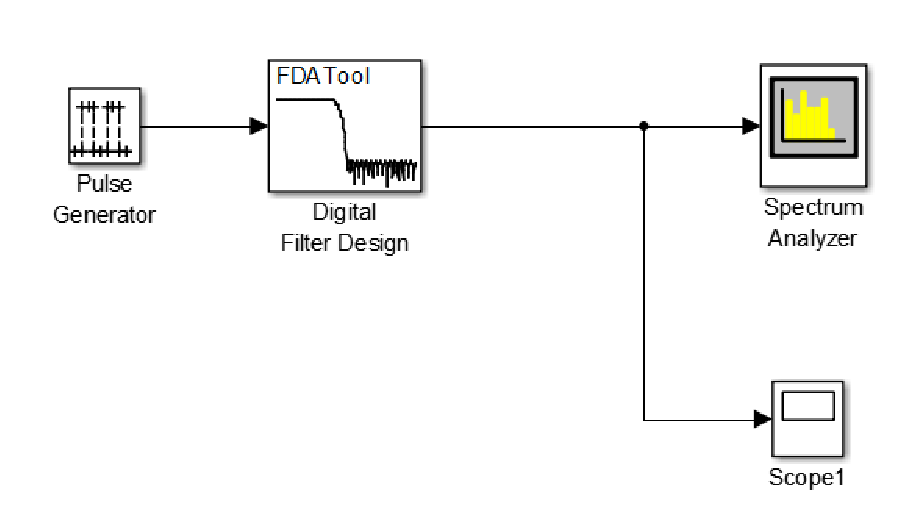
\includegraphics[width=10cm]{4_simulink} 
\caption{Треугольный импульсный сигнал (Simulink)} 
\label{fig.l5_7s} 
\end{figure}
\begin{figure}[h]
\centering
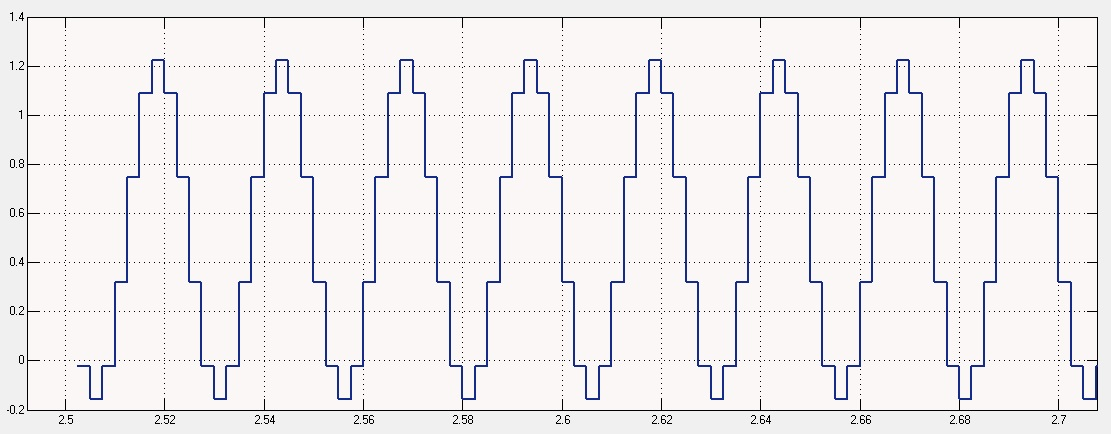
\includegraphics[width=10cm]{lab5_5_simulink} 
\caption{Треугольный импульсный сигнал} 
\label{fig.l5_8s} 
\end{figure}
\begin{figure}[h]
\centering
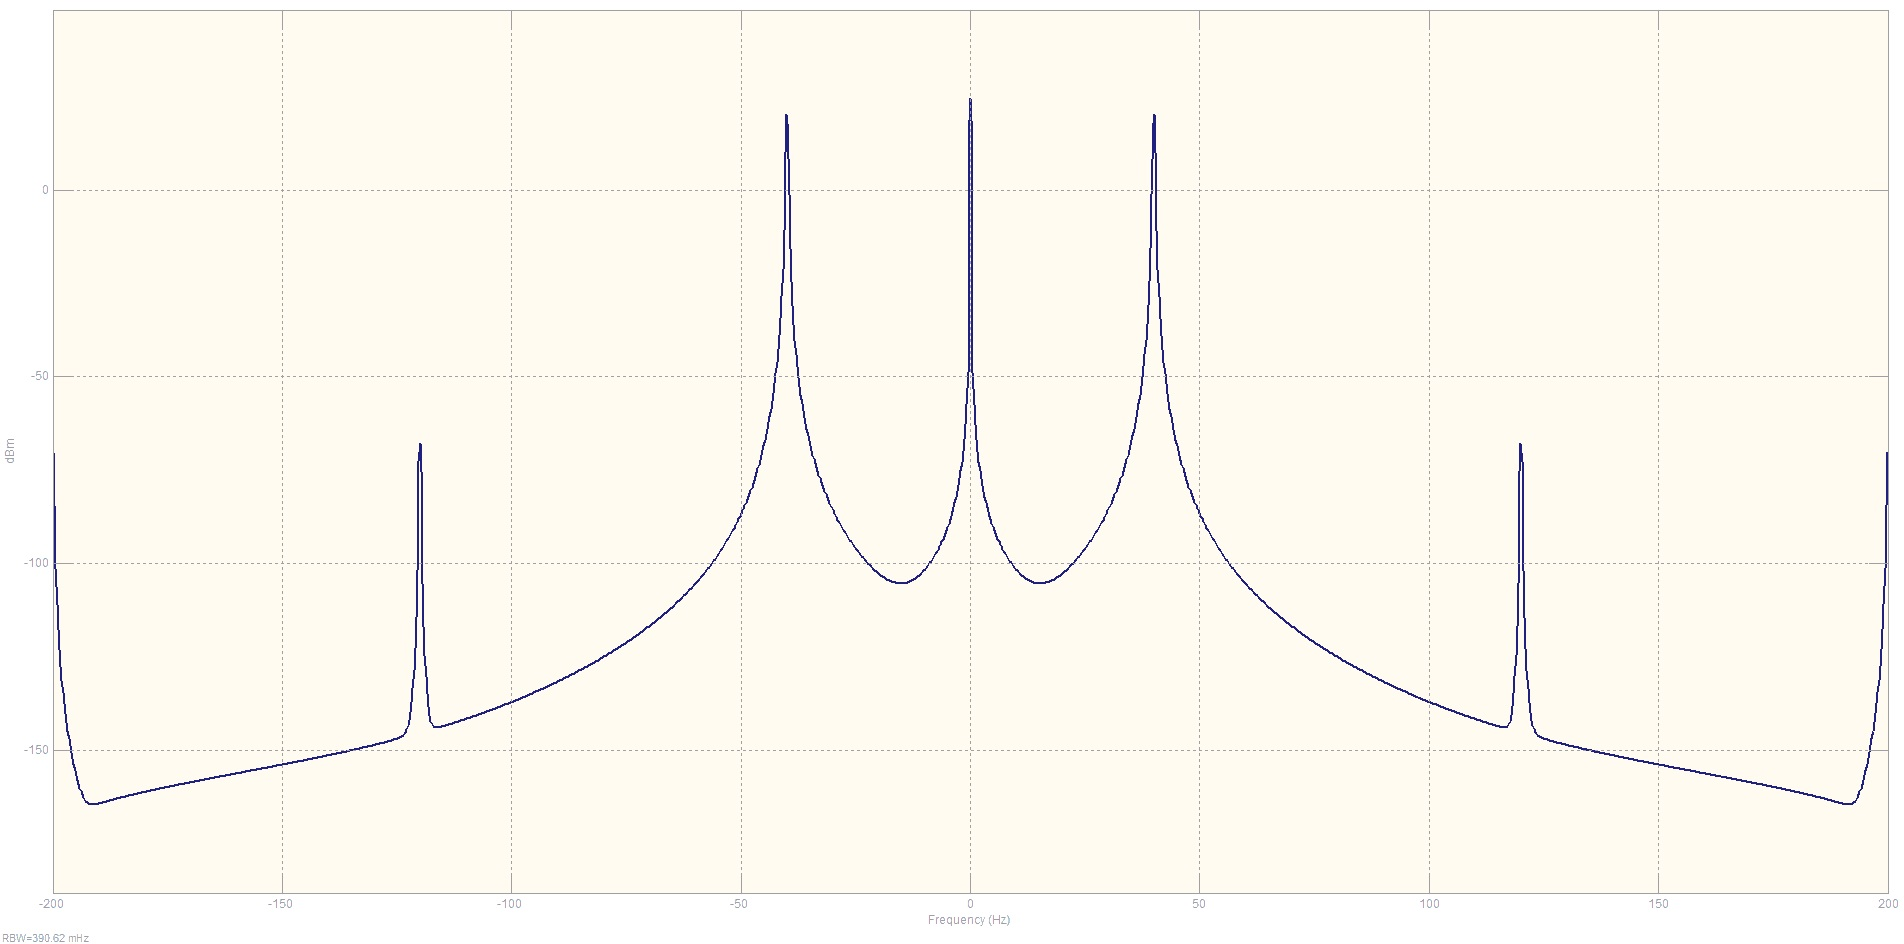
\includegraphics[width=10cm]{lab5_6_simulink}
\caption{Спектр треугольного сигнала} 
\label{fig.l5_9s} 
\end{figure}
\end{itemize}
\FloatBarrier
\subsection{Выводы}
В результате проделанной работы было проведено моделирование в среде MatLAB и Simulink полигармонического, прямоугольного и треугольного импульсных сигналаов, а также получены их спектры. В Simulink для получения генератора треугольного сигнала используется генератор прямоугольных импульсов каскадно с фильтром с прямоугольным окном. Это обоснуется тем, что свертка двух прямоугольных импульсов в результате дает треугольный.

\newpage
\section{Линейная фильтрация}

\subsection{Цель работы}
Изучить воздействие ФНЧ на тестовый сигнал с шумом.

\subsection{Постановка задачи}
Сгенерировать гармонический сигнал с шумом и синтезировать ФНЧ. Получить сигнал во временной и частотной областях до и после фильтрации. Сделать выводы о воздействии ФНЧ на спектр сигнала.

\subsection{Справочные материалы}
В.С. Гутников. Фильтрация измерительных сигналов пп. 17-19

\subsection{Ход работы}
Фильтрация сигнала - изменение его спектра, которое обычно применяется с целью увеличить отношение полезного сигнала к шумам и помехам или усилить какие-нибудь полезные качества сигнала.
В данной работе рассматривается фильтр нижних частот (ФНЧ), пропускающий низкочастотные составляющие спектра и задерживают высокочастотные, а именно фильтр Баттерворта с максимально гладкой АЧХ.  
Для моделирования заданных сигналов использовался приведенный ниже код MATLAB:
\begin{flushleft}

x = 0:0.01:4*pi;\\
f = 100*(0:255)/512;\\

noise = rand(size(x));\\
y = sin(2*pi*x);            \% Сигнал без шума\\
y\_noisy = y+0.3*noise;      \% Сигнал с шумом\\

figure\\
plot(x(1:200),y(1:200))\\
grid\\

figure\\
plot(x(1:200),y\_noisy(1:200))\\
grid\\

[B,A] = butter(16,0.98);    \% Синтез ФНЧ Баттерворта\\
B = B./sum(B);\\
A = A./sum(A);\\
                      
y\_filtered = conv(y\_noisy, [B, A]); \% Обработка сигнала ФНЧ\\

figure\\
plot(x(1:200),y\_filtered(1:200))\\
grid\\

noisy\_spectrum = fft(y\_noisy, 512); \% Спектр сигнала с шумом\\
norm\_noisy\_spectrum = noisy\_spectrum.*conj(noisy\_spectrum)/512;\\

figure\\
plot(f, norm\_noisy\_spectrum(1:256))\\
axis([0 max(f) 0 2])\\
grid \\

filtered\_spectrum = fft(y\_filtered, 512);   \% Спектр фильтрованного сигнала\\
norm\_filtered\_spectrum = filtered\_spectrum.*conj(filtered\_spectrum)/512;\\

figure\\
plot(f, norm\_filtered\_spectrum(1:256))\\
axis([0 max(f) 0 2])\\
grid\\


\end{flushleft}
\subsection{Результаты работы}
В результате работы представленного кода были получены следующие данные:

\begin{itemize}
\item Исходный гармонический сигнал (Рис. 20); 
\item Сигнал с шумом и его спектр (Рис. 21 - 22);
\item Отфильтрованный сигнал и его спектр (Рис. 23 - 24).
\end{itemize}

\begin{figure}[h]
\centering
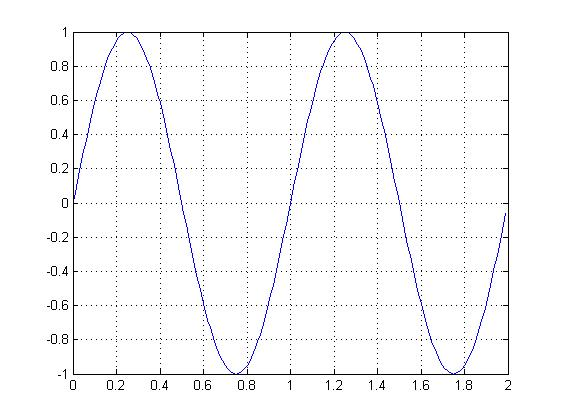
\includegraphics[width=6.5cm]{lab6_0} 
\caption{Исходный гармонический сигнал} 
\label{fig.l6_0} 
\end{figure}

\begin{figure}[h]\centering
  \parbox[b]{0.49\textwidth}{\centering
    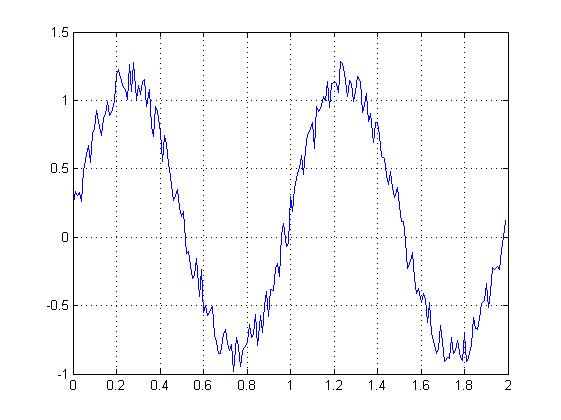
\includegraphics[width=6.5cm]{lab6_1} 
    \caption{Зашумленный гармонический сигнал}\label{fig.l6_1}}
  \hfil\hfil 
  \begin{minipage}[b]{0.49\textwidth}
	\centering
	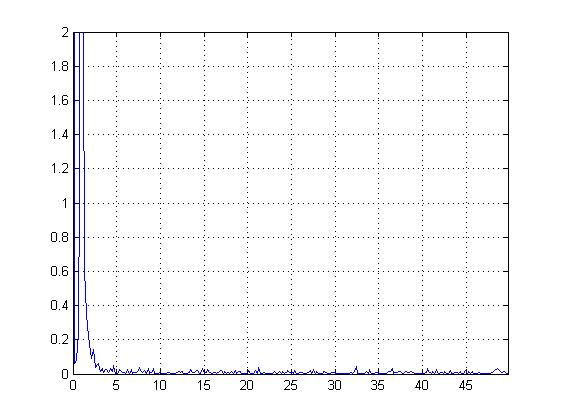
\includegraphics[width=6.5cm]{lab6_2}
	\caption{Спектр зашумленного сигнала}\label{fig.l6_2} 
  \end{minipage}
\end{figure}

\begin{figure}[h]\centering
  \parbox[b]{0.49\textwidth}{\centering
    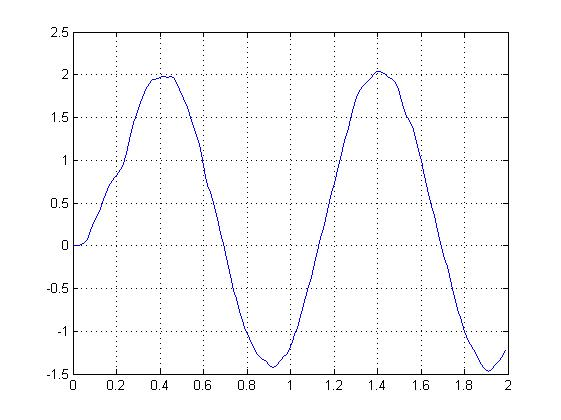
\includegraphics[width=6.5cm]{lab6_3} 
    \caption{Отфильтрованный сигнал}\label{fig.l6_3}}
  \hfil\hfil 
  \begin{minipage}[b]{0.49\textwidth}
	\centering
	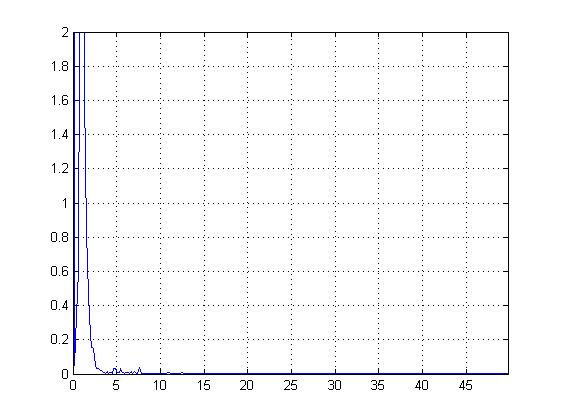
\includegraphics[width=6.5cm]{lab6_4}
	\caption{Спектр отфильтрованного сигнала}\label{fig.l6_4} 
  \end{minipage}
\end{figure}

\FloatBarrier
                                                                                                                                                                                                                                                                                                                                                                                                                                                                                                                                                                                                                                                                                                                                                                                                                                                                                                                                                                                                                                                                                                                                                                                                                                                                                                                                                                                                                                                                                                                                                                                                                                                                                                                                                                                                                                                                                                                                                                                                                                                                                                                                                                                                                                                                                                                                                                                                                                                                                                                                                                                                                                                                                                                                                                                                                                                                                                                                                                                                                                                                                                                                                                                                                                                                                                                                                                                                                                                                                                                                                                                                                                                                                                                                                                                                                                                                                                                                                                                                                                                                                                                                                                                                                                                              Аналогичное моделирование было проведено в среде Simulink (построенный блок отображен на Рис. 25). В результате были получены характеристики, представленные на Рис. 26 - 27.
                                                                                                                                                                                                                                                                                                                                                                                                                                                                                                                                                                                                                                                                                                                                                                                                                                                                                                                                                                                                                                                                                                                                                                                                                                                                                                                                                                                                                                                                                                                                                                                                                                                                                                                                                                                                                                                                                                                                                                                                                                                                                                                                                                                                                                                                                                                                                                                                                                                                                                                                                                                                                                                                                                                                                                                                                                                                                                                                                                                                                                                                                                                                                                                                                                                                                                                                                                                                                                                                                                                                                                                                                                                                                                                                                                                                                                                                                                                                                                                                                                                                                                                                                                                                                                                               \begin{figure}[h]\centering
	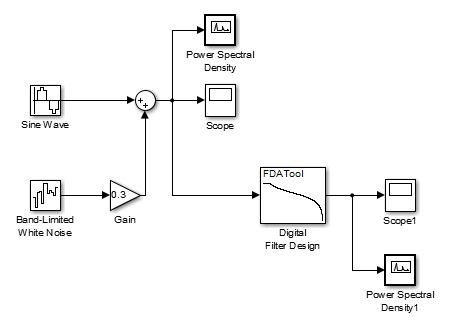
\includegraphics[width=10cm]{Sim_0} 
	\caption{Исходный гармонический сигнал}\label{fig.l6_Sim0} 
\end{figure}
                                                                                                                                                                                                                                                                                                                                                                                                                                                                                                                                                                                                                                                                                                                                                                                                                                                                                                                                                                                                                                                                                                                                                                                                                                                                                                                                                                                                                                                                                                                                                                                                                                                                                                                                                                                                                                                                                                                                                                                                                                                                                                                                                                                                                                                                                                                                                                                                                                                                                                                                                                                                                                                                                                                                                                                                                                                                                                                                                                                                                                                                                                                                                                                                                                                                                                                                                                                                                                                                                                                                                                                                                                                                                                                                                                                                                                                                                                                                                                                                                                                                                                                                                                                                                                                               \begin{figure}[h]\centering
    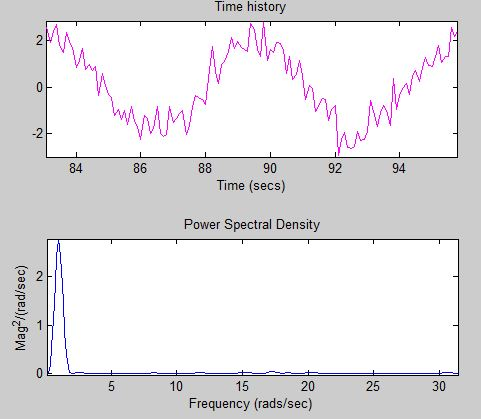
\includegraphics[width=10cm]{Sim_1} 
    \caption{Отфильтрованный сигнал}\label{fig.l6_Sim1}
\end{figure}

\begin{figure}\centering
	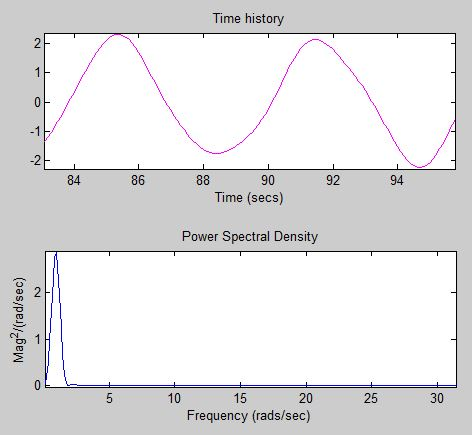
\includegraphics[width=10cm]{Sim_2}
	\caption{Спектр отфильтрованного сигнала}\label{fig.l6_Sim2}
\end{figure}                                                                                                                                                                                                                                                                                                                                                                                                                                                                                                                                                                                                                                                                                                                                                                                                                                                                                                                                                                                                                                                                                                                                                                                                                                                                                                                                                                                                                                                                        

\FloatBarrier

\subsection{Выводы}
В данной работе было изучено воздействие ФНЧ на тестовый сигнал с шумом, а именно произведено зашумление и удаление шума линейым фильтром Баттерворта. Однако фильтрация оказалась неполной. Это связано с тем, что использованный линейный фильтр не способен разделить шум и полезный сигнал в одной частотной области. Для полной фильтрации необходимо использовать идеальный фильтр с прямоугольным окном.

\newpage
\section{Аналоговая модуляция}

\subsection{Цель работы}
Изучение аналоговой модуляции/демодуляции сигнала.

\subsection{Постановка задачи}
	\begin{enumerate}
		\item Сгенерировать однотоальный сигнал низкой частоты.
		\item Выполнить амплитудную модуляцию сигнала по закону
				\begin{equation}
					u(t) = (1+MU_m cos(\Omega t))cos(\omega_0 t+\phi_0).
				\end{equation}
		\item Получить спектр модулированного сигнала.
		\item Выполнить модуляцию с подавлением несущей 
				\begin{equation}
					u(t) = MU_m cos(\omega t)cos(\omega_0 t+\phi_0).
				\end{equation}
		      Получить спектр. 
		\item Выполнить однополосную модуляцию:
				\begin{equation}
					u(t) = U_m cos(\omega t)cos(\omega_0 t+\phi_0)+\frac{U_m}{2}\sum_{n=1}^N M_n (cos(\omega_0 + \Omega_n )t + \phi_0 + \Phi_n ),
				\end{equation}
				положив n = 1.
		\item Выполить синхронное детектирование и получить исходный однополосный сигнал.
		\item Рассчитать КПД модуляции
				\begin{equation}
					\eta_A M = \frac{U_m ^2 M^2 /4}{P_U} = \frac{M^2}{M^2 + 2}.
				\end{equation}
	\end{enumerate}

\subsection{Справочные материалы}
Н.В. Богач и др. Обработка сигналов в информационных системах, с. 110-118, 125-127.

\subsection{Ход работы}
АМ - сигнал представляет собой произведение информационной огибающей u(t) и гармонического колебания ее заполнения с более высокими частотами. Простейшая форма модулированного сигнала создается при \textit{однотональной} АМ - модуляции несущего сигнала гармоническим колебанием с одной частотой $\Omega$:
	\begin{equation}
		u(t) = (1+MU_m cos(\Omega t))cos(\omega_0 t+\phi_0).
	\end{equation}

Реализация аналоговой модуляции с помощью MATLAB:
\begin{flushleft}
x = 0:0.01:4*pi;\\
f0 = 0.2;\\

\% Исходный сигнал\\
y = sin(2*pi*f0*x);\\
figure\\
plot(x(1:500),y(1:500), 'LineWidth', 2)\\
grid\\

\% Спектр исходного сигнала\\
spectrum = fft(y, 512);\\
norm\_spectrum = spectrum.*conj(spectrum)/512;\\
f = 100*(0:255)/512;\\
figure\\
plot(f, norm\_spectrum(1:256), 'LineWidth', 2)\\
axis([0 max(f) 0 40])\\
grid\\

\% Амплитудная модуляция\\
Fc = 5*f0;\\
Fs = 50*f0;\\
U = ammod(y, Fc, Fs, 0, 1);\\
figure \\
plot(x(1:500), U(1:500))\\
grid\\

\% Спектр модурированного сигнала\\
u\_spectrum = fft(U, 512);\\
norm\_u\_spectrum = u\_spectrum.*conj(u\_spectrum)/512;\\
figure\\
plot(f, norm\_u\_spectrum(1:256))\\
axis([0 max(f) 0 30])\\
grid\\
\end{flushleft}

В результате выполнения приведенного кода были получены следующие характеристики:

\begin{figure}[h]\centering
  \parbox[b]{0.49\textwidth}{\centering
    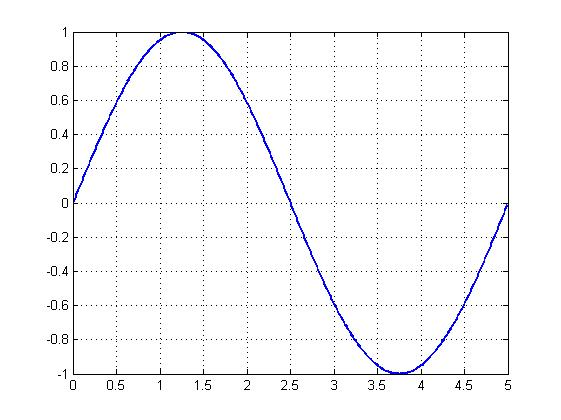
\includegraphics[width=6.5cm]{lab7_0} 
    \caption{Исходный гармонический сигнал}\label{fig.l7_0}}
  \hfil\hfil 
  \begin{minipage}[b]{0.49\textwidth}
	\centering
	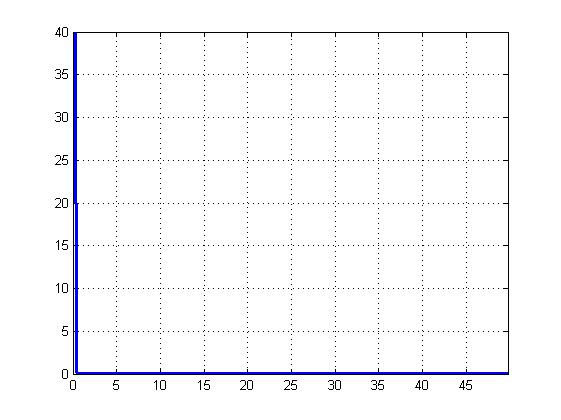
\includegraphics[width=6.5cm]{lab7_1}
	\caption{Спектр исходного сигнала}\label{fig.l7_1} 
  \end{minipage}
\end{figure}

\begin{figure}[h]\centering
  \parbox[b]{0.49\textwidth}{\centering
    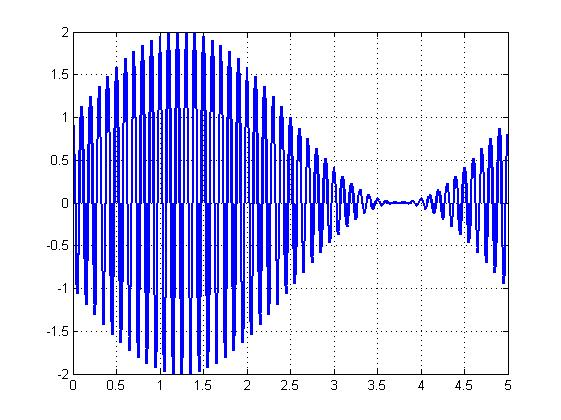
\includegraphics[width=6.5cm]{lab7_2} 
    \caption{Модуляция с М = 1}\label{fig.l7_2}}
  \hfil\hfil 
  \begin{minipage}[b]{0.49\textwidth}
	\centering
	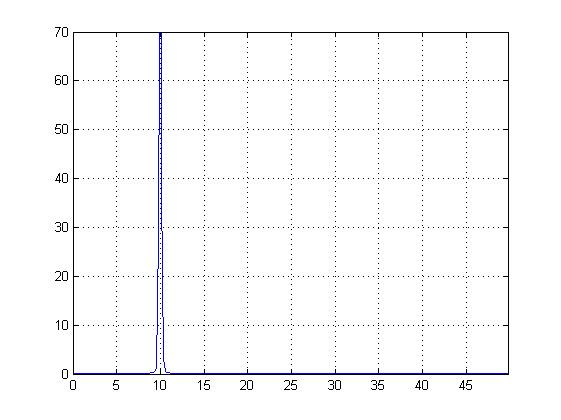
\includegraphics[width=6.5cm]{lab7_3}
	\caption{Спектр АМ-сигнала (М = 1)}\label{fig.l7_3} 
  \end{minipage}
\end{figure}

\begin{figure}[h]\centering
  \parbox[b]{0.49\textwidth}{\centering
    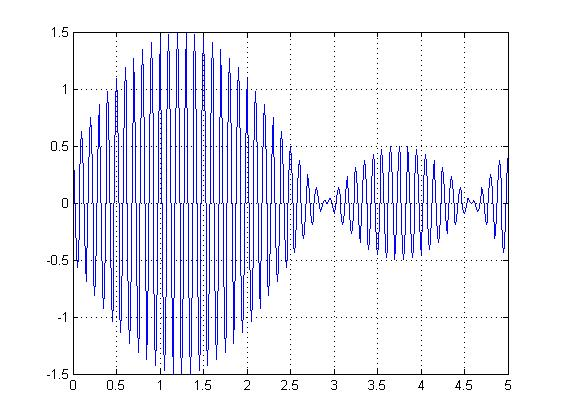
\includegraphics[width=6.5cm]{lab7_4} 
    \caption{Модуляция с М = 2}\label{fig.l7_4}}
  \hfil\hfil 
  \begin{minipage}[b]{0.49\textwidth}
	\centering
	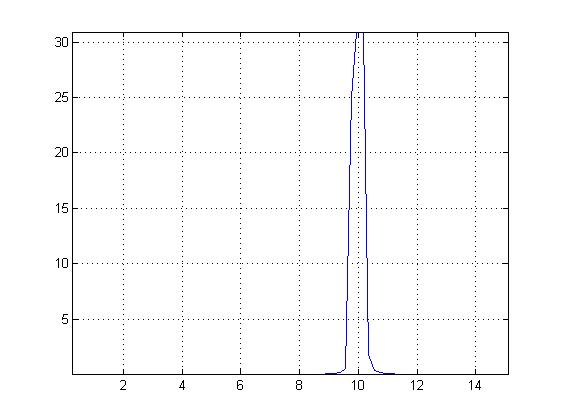
\includegraphics[width=6.5cm]{lab7_5}
	\caption{Спектр АМ-сигнала (М = 2)}\label{fig.l7_5} 
  \end{minipage}
\end{figure}

\begin{figure}[h]\centering
  \parbox[b]{0.49\textwidth}{\centering
    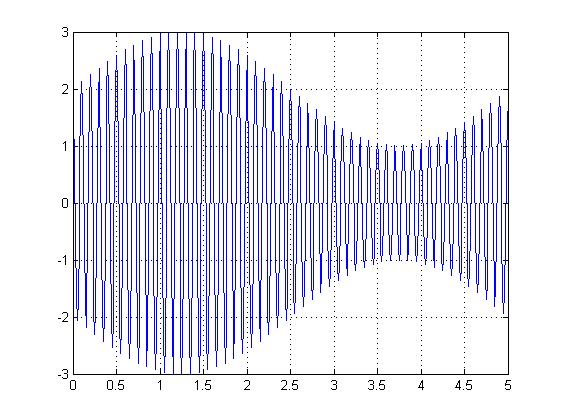
\includegraphics[width=6.5cm]{lab7_6} 
    \caption{Модуляция с М = 0.5}\label{fig.l7_6}}
  \hfil\hfil 
  \begin{minipage}[b]{0.49\textwidth}
	\centering
	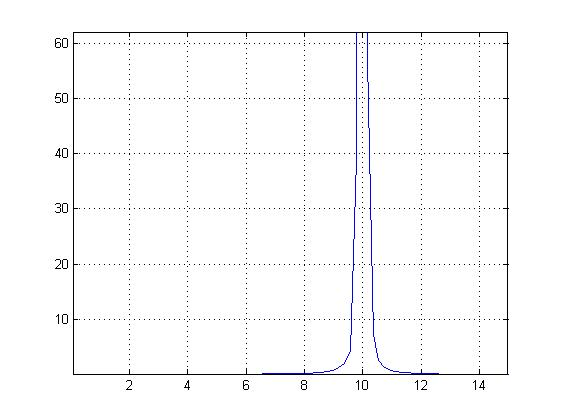
\includegraphics[width=6.5cm]{lab7_7}
	\caption{Спектр АМ-сигнала (М = 0.5)}\label{fig.l7_7} 
  \end{minipage}
\end{figure}

\FloatBarrier

При балансной модуляции (АМ с подавлением несущей) производится перемножение двух сигналов - модулирующего и несущего, при котором проиходит подавление неcущего колебания, соответственно, КПД модуляции становится равным 100\%. 
Физическая сущность подавления несущей заключается в том, что при переходе огибающей биений U(t) через 0 фаза несущей частоты высокочастотного заполнения изменяется на $180^0$.

Реализация аналоговой модуляции c подавлением несущей с помощью MATLAB:
\begin{flushleft}

\% Амплитудная модуляция с подавлением несущей\\
Fc = 10*f0;\\
Fs = 100*f0;\\
U = ammod(y, Fc, Fs);\\
figure \\
plot(x(1:500), U(1:500), 'LineWidth', 2)\\
grid\\

\% Спектр модурированного сигнала\\
u\_spectrum = fft(U, 512);
norm\_u\_spectrum = u\_spectrum.*conj(u\_spectrum)/512;\\
figure\\
plot(f, norm\_u\_spectrum(1:256))\\
axis([0 max(f) 0 30])\\
grid\\
\end{flushleft}

В результате выполнения приведенного кода были получены следующие характеристики:

\begin{figure}[h]\centering
  \parbox[b]{0.49\textwidth}{\centering
    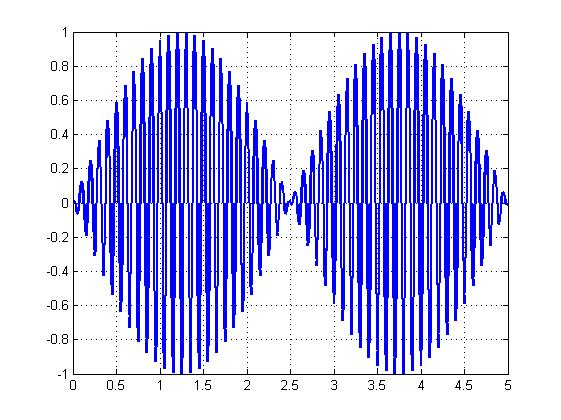
\includegraphics[width=6.5cm]{lab7_8} 
    \caption{АМ-сигнал с подавлением несущей}\label{fig.l7_8}}
  \hfil\hfil 
  \begin{minipage}[b]{0.49\textwidth}
	\centering
	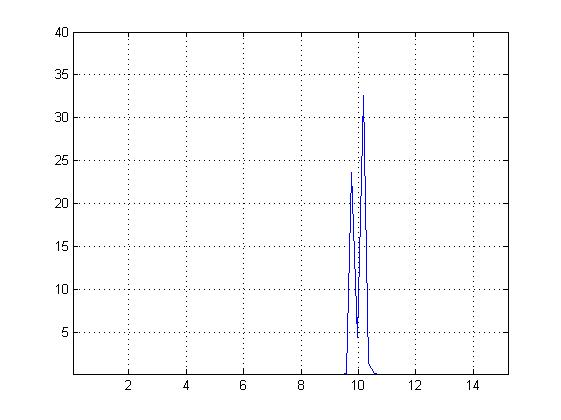
\includegraphics[width=6.5cm]{lab7_9}
	\caption{Спектр АМ-сигнала с подавлением}\label{fig.l7_9} 
  \end{minipage}
\end{figure}

\FloatBarrier

Спектры двух боковых полос АМ-сигнала являются зеркальным отражением друг друга, т.е. они несут одну и ту же информацию. Поэтому одну из боковых полос можно удалить.

Для этого был использван следующий код MATLAB:
\begin{flushleft}
\% Однополосная амплитудная модуляция\\
Fc = 10*f0;\\
Fs = 100*f0;\\
U = ssbmod(y, Fc, Fs, [], 'upper');\\
figure \\
plot(x(1:500), U(1:500), 'LineWidth', 2)\\
grid\\

\% Спектр модурированного сигнала\\
u\_spectrum = fft(U, 512);
norm\_u\_spectrum = u\_spectrum.*conj(u\_spectrum)/512;\\
figure\\
plot(f, norm\_u\_spectrum(1:256))\\
axis([0 max(f) 0 30])\\
grid\\
\end{flushleft}

В результате выполнения приведенного кода были получены следующие графики:

\begin{figure}[h]\centering
  \parbox[b]{0.49\textwidth}{\centering
    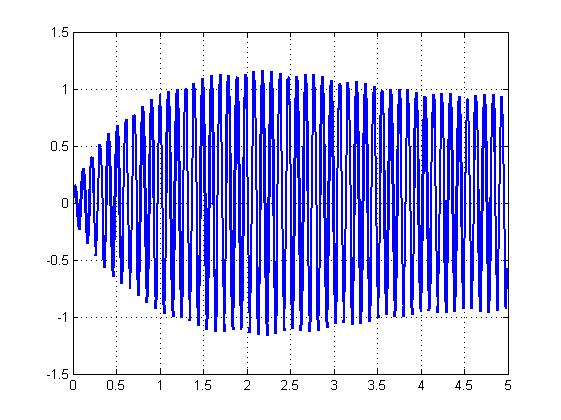
\includegraphics[width=6.5cm]{lab7_10} 
    \caption{Однополосный АМ-сигнал}\label{fig.l7_10}}
  \hfil\hfil 
  \begin{minipage}[b]{0.49\textwidth}
	\centering
	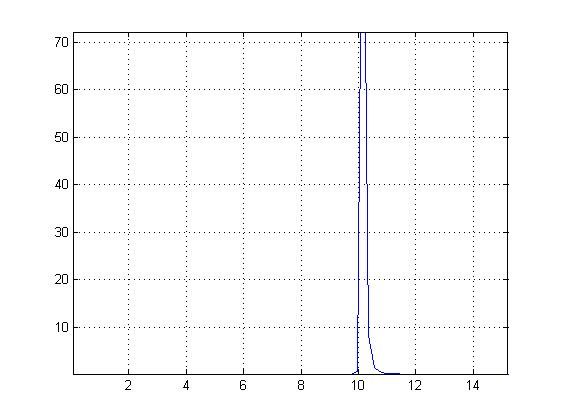
\includegraphics[width=6.5cm]{lab7_11}
	\caption{Спектр однополосного АМ-сигнала}\label{fig.l7_11} 
  \end{minipage}
\end{figure}

\FloatBarrier

Синхронное детектирование является одним из способов демодуляции АМ-сигнала. Его суть состоит в умножении частоты сигнала на опорное колебание с несущей частотой. Результат умножения содержит два слагаемых: искомая амплитуда и АМ-сигнал с несущей частотой $2\omega_0$, который легко удаляется путем пропускания сигнала через ФНЧ.

Ниже приведен реализующий синхронное детектирование код MATLAB:

\begin{flushleft}
\% Синхронное детектирование\\
%[b,a] = butter(10, Fc*2/Fs);\\
z = ssbdemod(U, Fc, Fs, 0, b, a);\\
figure\\
plot(x(1:1000), z(1:1000))\\
grid\\

\% Спектр демодулированного сигнала\\
du\_spectrum = fft(U, 512);\\
norm\_du\_spectrum = du\_spectrum.*conj(du\_spectrum)/512;\\
figure\\
plot(f, norm\_du\_spectrum(1:256))\\
axis([0 max(f) 0 70])\\
grid\\
\end{flushleft}

В результате синхронного дететирования демодулированный сигнал полностью совпал с исходным сигналом:

\begin{figure}[h]\centering
  \parbox[b]{0.49\textwidth}{\centering
    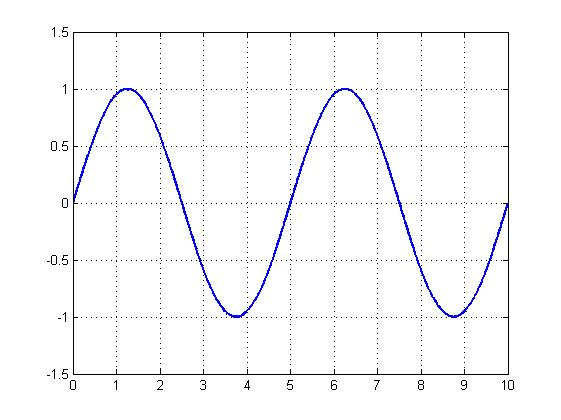
\includegraphics[width=6.5cm]{lab7_12} 
    \caption{Демодулированный АМ-сигнал}\label{fig.l7_12}}
  \hfil\hfil 
  \begin{minipage}[b]{0.49\textwidth}
	\centering
	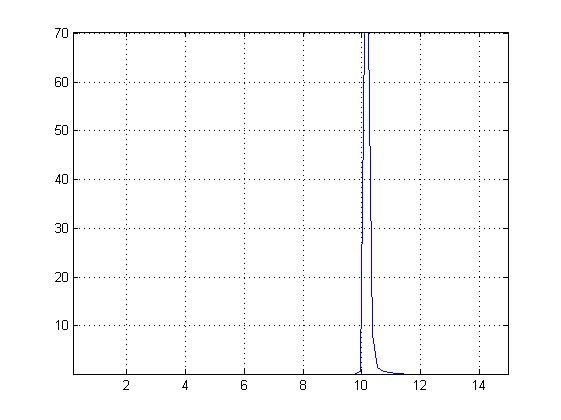
\includegraphics[width=6.5cm]{lab7_13}
	\caption{Спектр демодулированного сигнала}\label{fig.l7_13} 
  \end{minipage}
\end{figure}

\FloatBarrier

В ходе работы был рассчитан КПД модуляции при различных значениях глубины М:

\begin{itemize}
	\item M = 1:		0.33;
	\item M = 2:		0.67;
	\item M = 0.5:		0.11.
\end{itemize}

\textbf{Однополосная модуляция/демодуляция в среде Simulink}

Для моделирования амплитудной однополосной модуляции и демодуляции использовались блоки SSB AM Modulator/Demodulaor Passband. Результаты моделирования приведены на Рис. 42-45:

\begin{figure}[h]\centering
	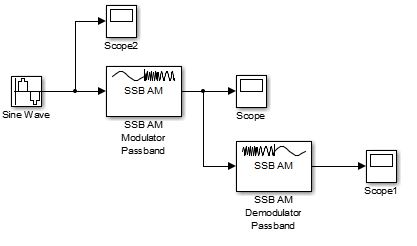
\includegraphics[width=6cm]{Sim_ssb0}
	\caption{Схема однополосной модуляции/демодуляции}\label{fig.Sim_ssb0}
\end{figure}                                                                                                                                                                                                                                                                                                                                                                                                                                                                                                                                                                                                                                                                                                                                                                                                                                                                                                                                                                                                                                                                                                                                                                                                                                                                                                                                                                                                                                                                        

\begin{figure}[h]\centering
	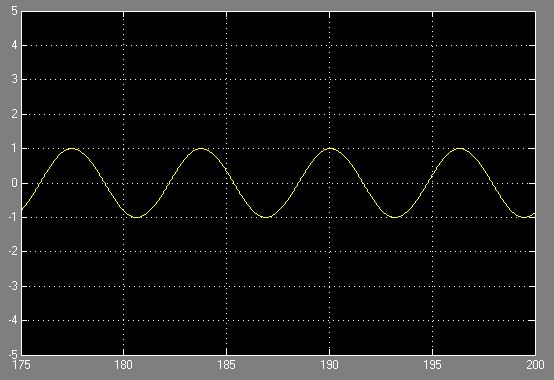
\includegraphics[width=8cm]{Sim_ssb1}
	\caption{Исходный сигнал}\label{fig.Sim_ssb1}
\end{figure}                                                                                                                                                                                                                                                                                                                                                                                                                                                                                                                                                                                                                                                                                                                                                                                                                                                                                                                                                                                                                                                                                                                                                                                                                                                                                                                                                                                                                                                                        

\begin{figure}[h]\centering
	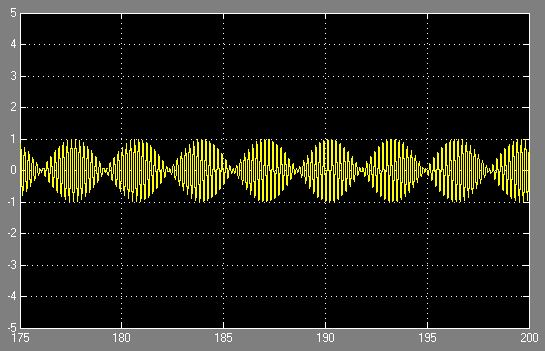
\includegraphics[width=8cm]{Sim_ssb2}
	\caption{АМ-сигнал}\label{fig.Sim_ssb2}
\end{figure}                                                                                                                                                                                                                                                                                                                                                                                                                                                                                                                                                                                                                                                                                                                                                                                                                                                                                                                                                                                                                                                                                                                                                                                                                                                                                                                                                                                                                                                                        

\begin{figure}[h]\centering
	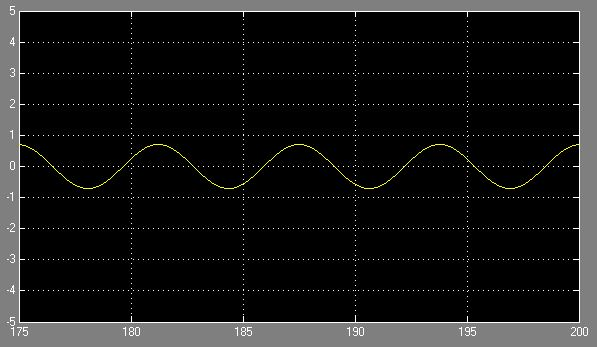
\includegraphics[width=8cm]{Sim_ssb3}
	\caption{Демодулированный АМ-сигнал}\label{fig.Sim_ssb3}
\end{figure}                                                                                                                                                                                                                                                                                                                                                                                                                                                                                                                                                                                                                                                                                                                                                                                                                                                                                                                                                                                                                                                                                                                                                                                                                                                                                                                                                                                                                                                                        

\FloatBarrier

Для моделирования балансной однополосной модуляции и демодуляции использовались блоки DSBSC AM Modulator/Demodulaor Passband. Исходный сигнал тот же (Рис. 43). Результаты моделирования приведены на Рис. 46-48:

\begin{figure}[h]\centering
	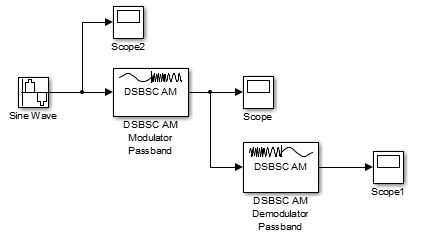
\includegraphics[width=6cm]{Sim_dsbsc0}
	\caption{Схема балансной модуляции/демодуляции}\label{fig.Sim_dsbsc0}
\end{figure}                                                                                                                                                                                                                                                                                                                                                                                                                                                                                                                                                                                                                                                                                                                                                                                                                                                                                                                                                                                                                                                                                                                                                                                                                                                                                                                                                                                                                                                                        

\begin{figure}[h]\centering
	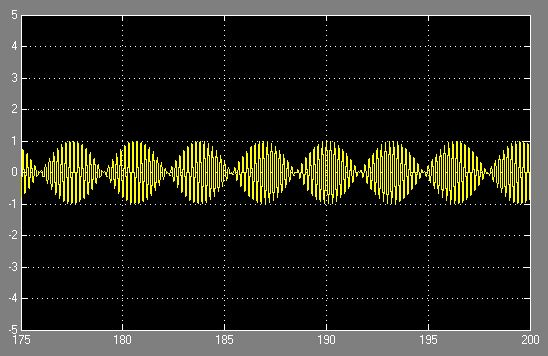
\includegraphics[width=8cm]{Sim_dsbsc2}
	\caption{БАМ-сигнал}\label{fig.Sim_dsbsc2}
\end{figure}                                                                                                                                                                                                                                                                                                                                                                                                                                                                                                                                                                                                                                                                                                                                                                                                                                                                                                                                                                                                                                                                                                                                                                                                                                                                                                                                                                                                                                                                        

\begin{figure}[h]\centering
	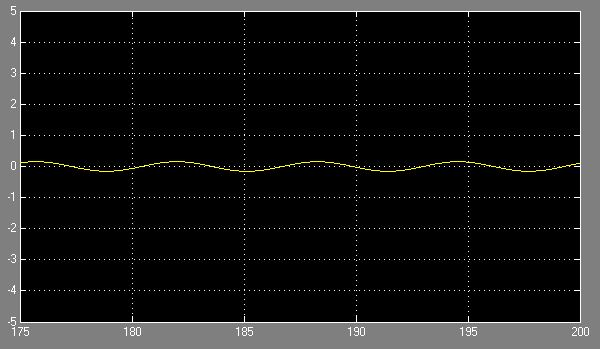
\includegraphics[width=8cm]{Sim_dsbsc3}
	\caption{Демодулированный БАМ-сигнал}\label{fig.Sim_dsbsc3}
\end{figure}                                                                                                                                                                                                                                                                                                                                                                                                                                                                                                                                                                                                                                                                                                                                                                                                                                                                                                                                                                                                                                                                                                                                                                                                                                                                                                                                                                                                                                                                        

\FloatBarrier

\subsection{Выводы}
В ходе выполнения лабораторной работы был сгенерирован однотоальный сигнал низкой частоты, выполнена АМ сигнала и получен спектр модулированного сигнала. Также была выполнена БАМ и однополосная АМ и получены их спектры. Произведено синхронное детектирование и получен исходный однополосный сигнал. Рассчитан КПД модуляции.

АМ применяется на сравнительно низких частотах (не выше коротких волн). Это обусловлено низким КПД использования энергии модулированных сигналов.

Ширина спектра АМ-сигнала с подавленной несущей, как  в случае с обычной АМ, в два раза больше, чем у модулирующего сигнала. Но при БАМ производится перемножение двух сигналов – модулирующего и несущего, при котором происходит подавление несущего колебания, соответственно, КПД модуляции становится равным 100\%. 

Двухполосная АМ с подавленной несущей имеет приемущества перед обычной АМ только в энергетическом плане - за счет устранения несущего колебанияю, ширина спектра при этом по-прежнему вдвое больше, чем у модулирующего сигнала. Однако спектры двух боковых полос АМ-сигнала являются зеркальным отражением друг друга, поэтому одну из боковых полос можно удалить.

Однополосный сигнал можно представить как сумму двух АМ-сигналов, несущие колебания которых имеют одну и ту же частоту, но сдвинуты по фазе относительно друг друга на $90^0$.

Синхронное детектирование является одним из способов демодуляции АМ-сигнала. Его суть состоит в умножении частоты сигнала на опорное колебание с несущей частотой. Результат умножения содержит два слагаемых: искомая амплитуда и АМ-сигнал с несущей частотой $2\omega_0$, который легко удаляется путем пропускания сигнала через ФНЧ. В нашем случае использовался фильтр Баттерворта.

\newpage
\section{Частотная и фазовая модуляция}

\subsection{Цель работы}
Изучение частотной и фазовой модуляции/демодуляции сигнала.

\subsection{Постановка задачи}
	\begin{enumerate}
		\item Сгенерировать однотоальный сигнал низкой частоты.
		\item Выполнить фазовую модуляцию/демодуляцию сигнала по закону
				\begin{equation}
					u(t) = U_m cos(\Omega t + ks(t)),
				\end{equation}
		используюя встроенную функцию MatLab pmmod, pmdemod.
		\item Получить спектр модулированного сигнала.
		\item Выполнить частотню модуляцию/демодуляцию по закону
				\begin{equation}
					u(t) = U_m cos(\omega_0 t + k \int_0^t s(t) dt + \phi_0),
				\end{equation}
		используюя встроенные функции MatLab fmmod, fmdemod.
	\end{enumerate}

\subsection{Справочные материалы}
Н.В. Богач и др. Обработка сигналов в информационных системах, с. 118-125, 127-133.

\subsection{Ход работы}
Фазовая модуляция – процесс изменения мгновенной фазы несущего колебания пропорционально изменению непрерывного информационного сигнала. Фазомодулированный сигнал s(t) имеет следующий вид:
	\begin{equation}
	s(t) = g(t) \sin[2 \pi f_c t + \varphi(t)],
	\end{equation}
где g(t) — огибающая сигнала; $\varphi(t)$ является модулирующим сигналом; $f_c$ — частота несущего сигнала; t — время.
В случае, когда информационный сигнал является дискретным, то говорят о фазовой манипуляции.

По характеристикам фазовая модуляция близка к частотной модуляции. В случае синусоидального модулирующего (информационного) сигнала, результаты частотной и фазовой модуляции совпадают.

Реализация фазовой модуляции/демодуляции с помощью MATLAB:
\begin{verbatim}
% Исходный сигнал
x = 0:0.01:4*pi;
y = sin(2*pi*x);

figure
subplot(4, 1, 1);
plot(x(1:500), y(1:500))
grid
title('Исходный сигнал')
 
% Фазовоя модуляция
Fs = 1000;                      % Частота дискретизации 
Fc = 4;                         % Несущая частота 
phasedev = pi/2;                % Девиация фазы для фазовой модуляции
pm_y = pmmod(x,Fc,Fs,phasedev); % Фазовая модуляция
subplot(4, 1, 2);
plot(x(1:500), pm_y(1:500))
grid
title('Фазовая модуляция')

spectrum = fft(pm_y, 512);      % Спектр фазовой модуляции
norm_spectrum = spectrum.*conj(spectrum)/512;  
f = 100*(0:255)/512;
subplot(4, 1, 3);
plot(f, norm_spectrum(1:256))
grid
title('Спектр фазовой модуляции')
axis([min(f) max(f) 0 max(norm_spectrum)]);

pdm_y = pmdemod(pm_y,Fc,Fs,phasedev); % Демодуляция
subplot(4, 1, 4);
plot(x, pdm_y)
grid
title('Фазовая демодуляция')
\end{verbatim}


В результате выполнения приведенного кода были получены следующие характеристики:

\begin{figure}[h]\centering
	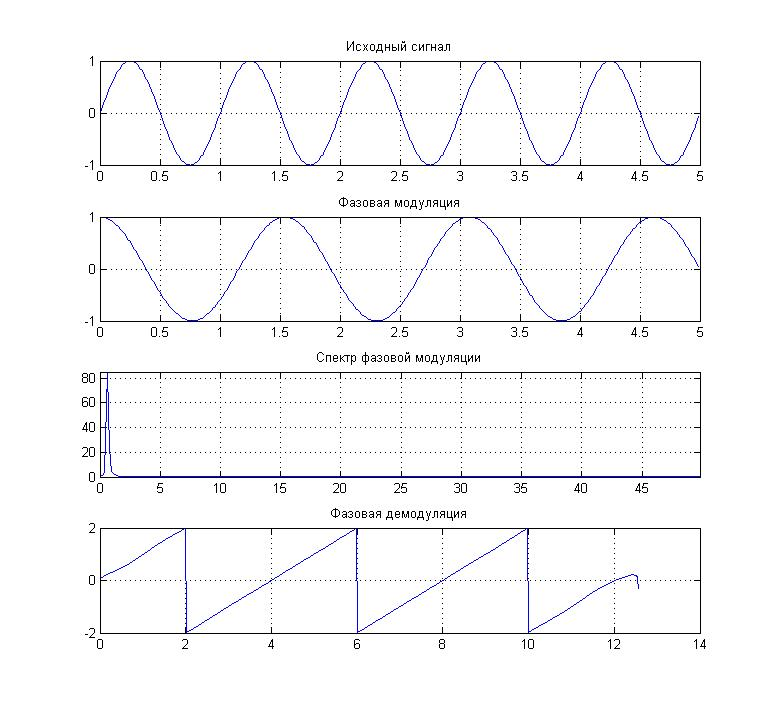
\includegraphics[width=10cm]{pm}
	\caption{Результаты фазовой модуляции/демодуляции}\label{fig.pm}
\end{figure}                                                                                                                                                                                                                                                                                                                                                                                                                                                                                                                                                                                                                                                                                                                                                                                                                                                                                                                                                                                                                                                                                                                                                                                                                                                                                                                                                                                                                                                                        
\FloatBarrier

Частотная модуляция – процесс изменения мгновенной частоты несущего колебания в соответствии с изменением информационного сигнала.По сравнению с амплитудной модуляцией здесь амплитуда остаётся постоянной.

Реализация частотной модуляции/демодуляции с помощью MATLAB:
\begin{verbatim}
% Исходный сигнал
x = 0:0.01:4*pi;
y = sin(2*pi*x);

figure
subplot(4, 1, 1);
plot(x(1:500), y(1:500))
grid
title('Исходный сигнал')
 
% Частотная модуляция
freqdev = 20;                	% Девиация частоты для частотной модуляции
fm_y = fmmod(x,Fc,Fs,freqdev); 	% Частотная модуляция
subplot(4, 1, 2);
plot(x(1:500), fm_y(1:500))
grid
title('Частотная модуляция')
spectrum = fft(fm_y, 512);      % Спектр частотной модуляции
norm_spectrum = spectrum.*conj(spectrum)/512;  
f = 100*(0:255)/512;
subplot(4, 1, 3);
plot(f, norm_spectrum(1:256))
grid
title('Спектр частотной модуляции')
axis([min(f) max(f) 0 max(norm_spectrum)]);
fdm_y = fmdemod(fm_y,Fc,Fs,freqdev); 	% Демодуляция
subplot(4, 1, 4);
plot(x, fdm_y)
grid
title('Частотная демодуляция')

\end{verbatim}


В результате выполнения приведенного кода были получены следующие характеристики:

\begin{figure}[h]\centering
	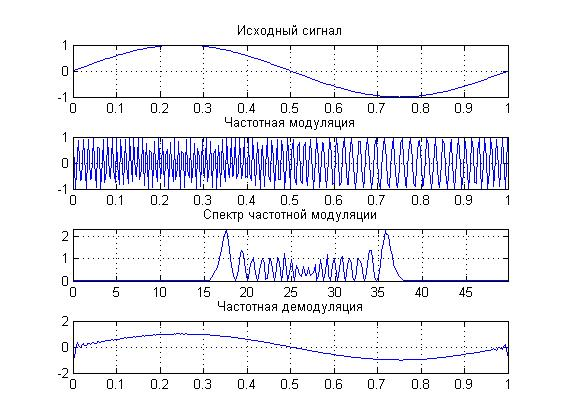
\includegraphics[width=10cm]{fm}
	\caption{Результаты частотной модуляции/демодуляции}\label{fig.fm}
\end{figure}                                                                                                                                                                                                                                                                                                                                                                                                                                                                                                                                                                                                                                                                                                                                                                                                                                                                                                                                                                                                                                                                                                                                                                                                                                                                                                                                                                                                                                                                        
\FloatBarrier

Для создания содели в Simulinc использовался раздел Communication Blockset Simulink. Выполнена модуляция, в том числе с помощью блока захваты фазы Phase-Locked Loop.

Для моделирования использоовался исходный сигнал, представленный на Рис. 51.

\begin{figure}[h]\centering
    \includegraphics[width=7cm]{sim_y} 
    \caption{Исходный сигнал}\label{fig.sim_y}
\end{figure}                                                                                                                                                                                                                                                                                                                                                                                                                                                                                                                                                                                                                                                                                                                                                                                                                                                                                                                                                                                                                                                                                                                                                                                                                                                                                                                                                                                                                                                                       
\FloatBarrier

Фазовая модуляция/демодуляция в Simulink:
\begin{figure}[h]\centering
    \includegraphics[width=7cm]{sim_p} 
    \caption{Фазовая модуляция/демодуляция}\label{fig.sim_p}
\end{figure}                                                                                                                                                                                                                                                                                                                                                                                                                                                                                                                                                                                                                                                                                                                                                                                                                                                                                                                                                                                                                                                                                                                                                                                                                                                                                                                                                                                                                                                                       

В результате были получены следующие характеристики:
\begin{figure}[h]\centering
  \parbox[b]{0.49\textwidth}{\centering
    \includegraphics[width=6.5cm]{sim_pm} 
    \caption{ФМ-сигнал}\label{fig.sim_pm}}
  \hfil\hfil 
  \begin{minipage}[b]{0.49\textwidth}
	\centering
	\includegraphics[width=6.5cm]{sim_pms}
	\caption{Спектр ФМ-сигнала}\label{fig.sim_pms} 
  \end{minipage}
\end{figure}

\begin{figure}[h]\centering
    \includegraphics[width=7cm]{sim_pdm} 
    \caption{Думодулированный ФМ-сигнал}\label{fig.sim_pdm}
\end{figure}
\FloatBarrier
\subsection{Выводы}

Частотная модуляция/демодуляция в Simulink:
\begin{figure}[h]\centering
    \includegraphics[width=7cm]{sim_f} 
    \caption{Частотная модуляция/демодуляция}\label{fig.sim_f}
\end{figure}                                                                                                                                                                                                                                                                                                                                                                                                                                                                                                                                                                                                                                                                                                                                                                                                                                                                                                                                                                                                                                                                                                                                                                                                                                                                                                                                                                                                                                                                       

В результате были получены следующие характеристики:
\begin{figure}[h]\centering
  \parbox[b]{0.49\textwidth}{\centering
    \includegraphics[width=6.5cm]{sim_fm} 
    \caption{ЧМ-сигнал}\label{fig.sim_fm}}
  \hfil\hfil 
  \begin{minipage}[b]{0.49\textwidth}
	\centering
	\includegraphics[width=6.5cm]{sim_fms}
	\caption{Спектр ЧМ-сигнала}\label{fig.sim_fms} 
  \end{minipage}
\end{figure}

\begin{figure}[h]\centering
    \includegraphics[width=7cm]{sim_fdm} 
    \caption{Думодулированный ЧМ-сигнал}\label{fig.sim_fdm}
\end{figure}
\FloatBarrier

Фазовая автоподстройка частоты — система автоматического регулирования, подстраивающая фазу управляемого генератора так, чтобы она была равна фазе опорного сигнала, либо отличалась на известную функцию от времени. Регулировка осуществляется благодаря наличию отрицательной обратной связи. Выходной сигнал управляемого генератора сравнивается на фазовом детекторе с опорным сигналом, результат сравнения используется для подстройки управляемого генератора.

Система ФАПЧ используется для частотной модуляции и демодуляции, умножения и преобразования частоты, частотной фильтрации, выделения опорного колебания для когерентного детектирования и в других целях.

ФАПЧ сравнивает фазы входного и опорного сигналов и выводит сигнал ошибки, соответствующий разности между этими фазами. Сигнал ошибки проходит далее через фильтр низких частот и используется в качестве управляющего для генератора, управляемого напряжением (ГУН), обеспечивающего отрицательную обратную связь. Если выходная частота отклоняется от опорной, то сигнал ошибки увеличивается, воздействуя на ГУН в сторону уменьшения ошибки. В состоянии равновесия выходной сигнал фиксируется на частоте опорного.

Также в схеме ФАПЧ включен фазовый детекто, которыйсравнивает фазы двух входных сигналов. Обычно, один из них генерируется генератором сигнала, управляемым напряжением, а второй берется из внешнего источника. ФД имеет два входа, управляющих стоящей за ним схемой подстройки частоты, задача которой сделать фазы сигналов одинаковыми.

Для ФАПЧ сигнал ошибки из ФД (значение найденной разности фаз) подается на сглаживающий фильтр (фильтр нижних частот). Сигнал с фильтра подается на управляемый напряжением генератор, частота(фаза) выходного сигнала которого зависит от напряжения на входе. Сигнал с генератора по цепи обратной связи поступает назад в детектор, замыкая контур ФАПЧ.

Частотная модуляция/демодуляция с фазовой автоподстройкой частоты в Simulink:
\begin{figure}[h]\centering
    \includegraphics[width=7cm]{sim_pll} 
    \caption{Частотная модуляция/демодуляция}\label{fig.sim_pll}
\end{figure}                                                                                                                                                                                                                                                                                                                                                                                                                                                                                                                                                                                                                                                                                                                                                                                                                                                                                                                                                                                                                                                                                                                                                                                                                                                                                                                                                                                                                                                                       

В результате были получены следующие характеристики:

\begin{figure}[h]\centering
    \includegraphics[width=7cm]{sim_fpll_filt} 
    \caption{Выход фльтра}\label{fig.sim_fpll_filt}
\end{figure}
\begin{figure}[h]\centering
  \parbox[b]{0.49\textwidth}{\centering
    \includegraphics[width=6.5cm]{sim_fpll_pd} 
    \caption{Выход фазового детектора}\label{fig.sim_fm}}
  \hfil\hfil 
  \begin{minipage}[b]{0.49\textwidth}
	\centering
	\includegraphics[width=6.5cm]{sim_fpll_vco}
	\caption{Выход ГУН}\label{fig.sim_fpll_vco} 
  \end{minipage}
\end{figure}

\FloatBarrier
\subsection{Выводы}
В результате выполнения данной работы были выполнены частотная и фазовая модуляция/демодуляция, а также чатотная демодуляция с  помощью блока захвата фазы. Можно сделать вывод, что частотная и фазовая модуляция очень тесно взаимосвязаны, поскольку обе они влияют на аргумент функции cos. Поэтому эти два вида модуляции имеют общее название — угловая модуляция.Сигнал с угловой модуляцией имеет вид колебания, начальная фаза которого зависит от времени:
	\begin{equation}
	s_(t) = A_0 cos(\omega0 t + j(t)).
	\end{equation}

Различие между фазовой и частотной модуляцией заключается лишь в том, как именно начальная фаза $j(t)$ связана с модулирующим сигналом.

Для демодуляции использовалась петля ФАПЧ, состоящая из перемножителя (используемого в качестве фазового детектора), фильтра нижних частот и генератора, управляемого напряжением (ГУН). Получаемый на выходе петли ФАПЧ сигнал пропорционален отклонению мгновенной частоты модулированного сигнала от несущей частоты, поэтому при демодуляции ФМ этот сигнал можно дополнительно проинтегрировать, чтобы получить начальную фазу сигнала.

\newpage
\section{Цифровая модуляция}

\subsection{Цель работы}
Изучение методов модуляции цировых сигналов.

\subsection{Постановка задачи}
	\begin{enumerate}
		\item Получить сигналы BPSK, PSK, OQPSK, genQAM, MSK, M-FSK модуляторов.
		\item Построить их сигнальые созвездия.
		\item Провести сравнение изученных методов модуляции цифровых сигналов.
	\end{enumerate}

\subsection{Справочные материалы}
Н.В. Богач и др. Обработка сигналов в информационных системах, с. 137-141.

\subsection{Ход работы}
Цифровая модуляция и демодуляция включают в себя две стадии. При модуляции цифровое сообщение сначала преобразуется в аналоговый модулирующий сигнал с помощью функции modmap, а затем осуществляется аналоговая модуляция. При демодуляции сначала получается аналоговый демодулированный сигнал, а затем он преобразуется в цифровое сообщение с помощью функции demodmap.

Аналоговый несущий сигнал модулируется цифровым битовым потоком.
Существуют три фундаментальных типа цифровой модуляции (или шифтинга) и один гибридный:
\begin{enumerate}
    \item ASK – Amplitude shift keying (Амплитудная двоичная модуляция).
    \item FSK – Frequency shift keying (Частотая двоичная модуляция).
    \item PSK – Phase shift keying (Фазовая двоичная модуляция).
    \item ASK/PSK.
\end{enumerate}
Одна из частных реализаций схемы ASK/PSK, которая называется QAM - Quadrature Amplitude Modulation (квадратурная амплитудная модуляция (КАМ). Это метод объединения двух AM-сигналов в одном канале. Он позваляет удвоить эффективную пропускную способность. В QAM используется две несущих с одинаковой частотой но с разницей в фазе на четверть периода (отсюда и возникает слово квадратура). 
Частотная модуляция представляет логическую единицу интервалом с большей частотой, чем ноль.
Фазовый шифтинг представляет «0» как сигнал без сдвига, а «1» как сигнал со сдвигом.

BPSK : используется единственный сдвиг фазы между «0» и «1» — 180 градусов, половина периода.
Существуют также QPSK:
QPSK использует 4 различных сдвига фазы (по четверти периода) и может кодировать 2 бита в символе (01, 11, 00, 10). 

Реализация различных типов модуляций с помощью MATLAB:
\begin{verbatim}
%BPSK modulation
h = modem.pskmod('M', 2);
g = modem.pskdemod('M', 2);
msg = randint(10,1,2)
modSignal = modulate(h,msg);
errSignal = (randerr(1,10, 3) ./ 30)';
modSignal = modSignal + errSignal;
demodSignal = demodulate(g,modSignal);
figure
subplot(3, 1, 1)
plot(1:10, msg(1:10))
title('Сообщение')
subplot(3, 1, 2)
plot(1:10, modSignal(1:10))
title('Модулированный сигнал')
subplot(3, 1, 3)
plot(1:10, modSignal(1:10))
title('Демодулированный сигнал')
scatterplot(modSignal);
\end{verbatim}
\begin{figure}[h]\centering
	\includegraphics[width=10cm]{bpsk}
	\caption{BPSK}\label{fig.bpsk}
\end{figure}                                                                                                                                                                                                                                                                                                                                                                                                                                                                                                                                                                                                                                                                                                                                                                                                                                                                                                                                                                                                                                                                                                                                                                                                                                                                                                                                                                                                                                                                        
\begin{figure}[h]\centering
	\includegraphics[width=10cm]{BPSKm}
	\caption{Сигнальное созвездие BPSK}\label{fig.BPSKm}
\end{figure}                                                                                                                                                                                                                                                                                                                                                                                                                                                                                                                                                                                                                                                                                                                                                                                                                                                                                                                                                                                                                                                                                                                                                                                                                                                                                                                                                                                                                                                                        
\begin{figure}[h]\centering
	\includegraphics[width=10cm]{BPSKe}
	\caption{Глазковая диаграмма BPSK}\label{fig.BPSKe}
\end{figure}                                                                                                                                                                                                                                                                                                                                                                                                                                                                                                                                                                                                                                                                                                                                                                                                                                                                                                                                                                                                                                                                                                                                                                                                                                                                                                                                                                                                                                                                        
\FloatBarrier
\begin{verbatim}
%PSK modulation
h = modem.pskmod('M', 8);
g = modem.pskdemod('M', 8);
msg = randint(10,1,8);
modSignal = modulate(h,msg);
errSignal = (randerr(1,10, 3) ./ 30)';
modSignal = modSignal + errSignal;
demodSignal = demodulate(g,modSignal);
figure
subplot(3, 1, 1)
plot(1:10, msg(1:10))
title('Сообщение')
subplot(3, 1, 2)
plot(1:10, modSignal(1:10))
title('Модулированный сигнал')
subplot(3, 1, 3)
plot(1:10, modSignal(1:10))
title('Демодулированный сигнал')
scatterplot(modSignal);
\end{verbatim}
\begin{figure}[h]\centering
	\includegraphics[width=10cm]{psk}
	\caption{PSK}\label{fig.psk}
\end{figure}                                                                                                                                                                                                                                                                                                                                                                                                                                                                                                                                                                                                                                                                                                                                                                                                                                                                                                                                                                                                                                                                                                                                                                                                                                                                                                                                                                                                                                                                        
\begin{figure}[h]\centering
	\includegraphics[width=10cm]{PSKm}
	\caption{Сигнальное созвездие PSK}\label{fig.PSKm}
\end{figure}                                                                                                                                                                                                                                                                                                                                                                                                                                                                                                                                                                                                                                                                                                                                                                                                                                                                                                                                                                                                                                                                                                                                                                                                                                                                                                                                                                                                                                                                        
\begin{figure}[h]\centering
	\includegraphics[width=10cm]{PSKe}
	\caption{Глазковая диаграмма PSK}\label{fig.PSKe}
\end{figure}                                                                                                                                                                                                                                                                                                                                                                                                                                                                                                                                                                                                                                                                                                                                                                                                                                                                                                                                                                                                                                                                                                                                                                                                                                                                                                                                                                                                                                                                        
\FloatBarrier
\begin{verbatim}
%OQPSK modulation
h = modem.oqpskmod;
g = modem.oqpskdemod;
msg = randint(200,1,4);
modSignal = modulate(h,msg);
errSignal = (randerr(1,400, 100) ./ 30)';
modSignal = modSignal + errSignal;
demodSignal = demodulate(g,modSignal);
figure
subplot(3, 1, 1)
plot(1:200, msg(1:200))
title('Сообщение')
subplot(3, 1, 2)
plot(1:200, modSignal(1:200))
title('Модулированный сигнал')
subplot(3, 1, 3)
plot(1:200, modSignal(1:200))
title('Демодулированный сигнал')
scatterplot(modSignal);
\end{verbatim}
\begin{figure}[h]\centering
	\includegraphics[width=10cm]{oqpsk}
	\caption{OQPSK}\label{fig.oqpsk}
\end{figure}
\begin{figure}[h]\centering
	\includegraphics[width=10cm]{OQPSKm}
	\caption{Сигнальное созвездие OQPSK}\label{fig.OQPSKm}
\end{figure}                                                                                                                                                                                                                                                                                                                                                                                                                                                                                                                                                                                                                                                                                                                                                                                                                                                                                                                                                                                                                                                                                                                                                                                                                                                                                                                                                                                                                                                                        
\begin{figure}[h]\centering
	\includegraphics[width=10cm]{OQPSKe}
	\caption{Глазковая диаграмма OQPSK}\label{fig.OQPSKe}
\end{figure}                                                                                                                                                                                                                                                                                                                                                                                                                                                                                                                                                                                                                                                                                                                                                                                                                                                                                                                                                                                                                                                                                                                                                                                                                                                                                                                                                                                                                                                                        
\FloatBarrier
\begin{verbatim}
%GENQAM modulation
M = 10;
h = modem.genqammod('Constellation', exp(j*2*pi*[0:M-1]/M));
g = modem.genqamdemod('Constellation', exp(j*2*pi*[0:M-1]/M));
msg = randint(10,1,8);
modSignal = modulate(h,msg);
errSignal = (randerr(1,10, 3) ./ 30)';
modSignal = modSignal + errSignal;
demodSignal = demodulate(g,modSignal);
subplot(3, 1, 1)
plot(1:10, msg(1:10))
title('Сообщение')
subplot(3, 1, 2)
plot(1:10, modSignal(1:10))
title('Модулированный сигнал')
subplot(3, 1, 3)
plot(1:10, modSignal(1:10))
title('Демодулированный сигнал')
scatterplot(modSignal);
\end{verbatim}
\begin{figure}[h]\centering
	\includegraphics[width=10cm]{genqam}
	\caption{genQAM}\label{fig.genqam}
\end{figure}
\begin{figure}[h]\centering
	\includegraphics[width=10cm]{genQAMm}
	\caption{Сигнальное созвездие genQAM}\label{fig.genQAMm}
\end{figure}                                                                                                                                                                                                                                                                                                                                                                                                                                                                                                                                                                                                                                                                                                                                                                                                                                                                                                                                                                                                                                                                                                                                                                                                                                                                                                                                                                                                                                                                        
\begin{figure}[h]\centering
	\includegraphics[width=10cm]{genQAMe}
	\caption{Глазковая диаграмма genQAM}\label{fig.genQAMe}
\end{figure}                                                                                                                                                                                                                                                                                                                                                                                                                                                                                                                                                                                                                                                                                                                                                                                                                                                                                                                                                                                                                                                                                                                                                                                                                                                                                                                                                                                                                                                                        
\FloatBarrier
\begin{verbatim}
%MSK modulation
h = modem.mskmod('SamplesPerSymbol', 10);
g = modem.mskdemod('SamplesPerSymbol', 10);
msg = randint(10,1,2);
modSignal = modulate(h, msg);
errSignal = (randerr(1,100, 3) ./ 30)';
modSignal = modSignal + errSignal;
demodSignal = demodulate(g, modSignal);
subplot(3, 1, 1)
plot(1:10, msg(1:10))
title('Сообщение')
subplot(3, 1, 2)
plot(1:10, modSignal(1:10))
title('Модулированный сигнал')
subplot(3, 1, 3)
plot(1:10, modSignal(1:10))
title('Демодулированный сигнал')
scatterplot(modSignal);
\end{verbatim}
\begin{figure}[h]\centering
	\includegraphics[width=10cm]{msk}
	\caption{MSK}\label{fig.msk}
\end{figure}
\begin{figure}[h]\centering
	\includegraphics[width=10cm]{MSKm}
	\caption{Сигнальное созвездие MSK}\label{fig.MSKm}
\end{figure}                                                                                                                                                                                                                                                                                                                                                                                                                                                                                                                                                                                                                                                                                                                                                                                                                                                                                                                                                                                                                                                                                                                                                                                                                                                                                                                                                                                                                                                                        
\begin{figure}[h]\centering
	\includegraphics[width=10cm]{MSKe}
	\caption{Глазковая диаграма MSK}\label{fig.MSKe}
\end{figure}                                                                                                                                                                                                                                                                                                                                                                                                                                                                                                                                                                                                                                                                                                                                                                                                                                                                                                                                                                                                                                                                                                                                                                                                                                                                                                                                                                                                                                                                        
\FloatBarrier

Cоздания моделей в Simulink.

Для создания моделей в Simulink использовался рздел Communication Blockset/Digital Baseband/Passband Modulation.
\begin{figure}[h]\centering
	\includegraphics[width=10cm]{sim}
	\caption{Модель в Simulink}\label{fig.sim}
\end{figure}

В результате были получены следующие характеристики:

\begin{figure}[h]\centering
	\includegraphics[width=10cm]{BPSKs}
	\caption{BPSK}\label{fig.BPSKs}
\end{figure}
\begin{figure}[h]\centering
	\includegraphics[width=10cm]{PSKs}
	\caption{PSK}\label{fig.PSKs}
\end{figure}
\begin{figure}[h]\centering
	\includegraphics[width=10cm]{OQPSKs}
	\caption{OQPSK}\label{fig.OQPSKs}
\end{figure}
\begin{figure}[h]\centering
	\includegraphics[width=10cm]{genQAMs}
	\caption{genQAM}\label{fig.genQAMs}
\end{figure}
\begin{figure}[h]\centering
	\includegraphics[width=10cm]{MFSKs}
	\caption{M-FSK}\label{fig.MFSKs}
\end{figure}

\FloatBarrier
\subsection{Выводы}
В ходе выполнения даной работы были получены сигналы BPSK, PSK, OQPSK, genQAM, MSK, M-FSK модуляторов, построены их сигнальые созвездия и глазковые диаграммы, проведено их сравнение, по результатам которого можно сделать вывод, что чем выше уровень модуляции, тем большими скоростными возможностями и меньшей помехоустойчивостью она обладает и чем выше уровень модуляции, тем больше данных мы можем передать за единицу времени. А благодаря сигнальным созвездиям можно произвести оценку ошибки фазы и амплитуды анализируемого сигнала.

\end{document}
